%% Accounting Integrity in Metered LLM-Serving Infrastructure -- ACM Transactions on
%% AI Security and Privacy (TAISAP) submission.
%% Migrated from the FGCS (Elsevier) source; see CHANGELOG_TAISAP.md for the full diff.
%% Compiled with tectonic (XeTeX), acmart class (official ACM LaTeX template, manuscript+review).
\documentclass[manuscript,review]{acmart}

\usepackage[T1]{fontenc}
\usepackage{tikz}
\usetikzlibrary{positioning,arrows.meta,calc}
\PassOptionsToPackage{hyphens}{url}
\usepackage{xurl}
\graphicspath{{../results/figures/}{figures_cose/}}

\emergencystretch=2em

%% Rights-management metadata (acmDOI, acmISBN, copyright year, article number) is
%% intentionally absent -- ACM assigns this post-acceptance, not at submission.

\begin{document}

\title{Accounting Integrity in Metered LLM-Serving Infrastructure:
Bounded Evidence for Client-Side Under-Payment}

\author{Hardik}
\authornote{Corresponding author.}
\orcid{0009-0001-1642-6669}
\affiliation{%
  \institution{Department of Computer Science and Data Analytics, Indian Institute of
  Technology Patna}
  \country{India}
}
\affiliation{%
  \institution{Vivekananda Institute of Professional Studies -- Technical Campus}
  \city{New Delhi}
  \country{India}
}
\email{hardik_24a12res263@iitp.ac.in}

\author{Natasha Kaila}
\orcid{0009-0006-4252-9705}
\affiliation{%
  \institution{Vivekananda Institute of Professional Studies -- Technical Campus}
  \city{New Delhi}
  \country{India}
}
\email{09617711924_aids@vipstc.edu.in}

\begin{abstract}
Metered AI-inference services are deployed systems in which computational value is
streamed to the client before the charge is settled, usage is produced at runtime, and
settlement is often asynchronous -- placing the usage-metering and billing boundary
inside the security perimeter of the AI-serving infrastructure itself, not outside it.
We study the integrity of that boundary against an authenticated client that seeks to
pay less than it owes for inference it received. Modeling a metered request as a
lifecycle with a single integrity property, $V(r) \le N(r)$, we localize failures to
three architectural placements: state synchronization (B0), commitment timing (M1), and
usage authority (M2). We apply bounded exhaustive model checking in TLA+/TLC across ten
configurations and four invariants, and validate the model predictions on a testbed spanning three
execution topologies, three accounting families including an asynchronous event
pipeline, and a third-party serving stack. Three results follow. Reservation and
abort-safe finalization are orthogonal security properties: each secures only one of
solvency and accounting integrity, and only their conjunction secures both. Correct
usage computation does not imply correct billing: an architecture that recounts usage
accurately but bills the client-declared value leaks 58.3\% of delivered value in a
controlled setting and 69.0\% against a real serving stack, while server-authoritative
billing eliminates the leak. Asynchronous settlement reproduces over-serving under
strictly sequential arrivals with no concurrency at all, showing that the
synchronization condition concerns not concurrency but whether authorization is
atomically coupled to economic commitment on the authorizing path; this persists under a
network-separated two-machine deployment, while a settlement-confirmed serialization
control shows none. We state model-level security conditions separately from the
implementation patterns that satisfy them, report that the strongest defense against
usage-authority manipulation costs under 0.1\% of end-to-end time with real inference,
and delimit the formal model, extended with a second, causal-ordering specification of
the asynchronous settlement mechanism. The contribution is a systematic security
analysis of deployed AI-serving infrastructure: B0 is a
known baseline, and M1/M2 systematize, formalize, and measure mechanisms with prior
individual precedent.
\end{abstract}

\begin{CCSXML}
<ccs2012>
<concept>
<concept_id>10002978.10003006</concept_id>
<concept_desc>Security and privacy~Systems security</concept_desc>
<concept_significance>500</concept_significance>
</concept>
<concept>
<concept_id>10002978.10002986</concept_id>
<concept_desc>Security and privacy~Formal methods and theory of security</concept_desc>
<concept_significance>500</concept_significance>
</concept>
<concept>
<concept_id>10002978.10003006.10003013</concept_id>
<concept_desc>Security and privacy~Distributed systems security</concept_desc>
<concept_significance>300</concept_significance>
</concept>
<concept>
<concept_id>10002978.10003029.10003031</concept_id>
<concept_desc>Security and privacy~Economics of security and privacy</concept_desc>
<concept_significance>100</concept_significance>
</concept>
</ccs2012>
\end{CCSXML}

\ccsdesc[500]{Security and privacy~Systems security}
\ccsdesc[500]{Security and privacy~Formal methods and theory of security}
\ccsdesc[300]{Security and privacy~Distributed systems security}
\ccsdesc[100]{Security and privacy~Economics of security and privacy}

\keywords{LLM serving infrastructure, AI-system security, usage metering, distributed
accounting, asynchronous settlement, formal verification, TLA+, cloud billing integrity}

\maketitle

\section{Introduction}
\label{sec:intro}
LLM inference APIs bill for tokens that are produced at runtime and streamed to the
client before the charge is settled, which places the metering and billing path inside
the attack surface of the AI-serving system. The billed unit, the
token, is produced at runtime by an opaque, streamed, long-running computation delivered
to a remote client over a network; the quantity is a multi-category vector; and the
usage record that determines the charge is itself produced by the serving system while
the response is still in flight -- so the authorization, execution, and settlement paths
carry security-critical state, making the usage-metering and settlement
subsystem part of the AI-serving system's security boundary rather than a peripheral
accounting concern external to it. Mistakes in how that state is
partitioned across components can produce integrity failures even when every individual
component computes usage correctly, which is why this paper studies the accounting
lifecycle itself: its states, its transitions, the conditions under which it is safe, and
what happens empirically when those conditions are broken.

This is a structural property of metered computational services generally, not an
accident of one implementation, which is why the lifecycle we study is stated over the
request lifecycle of a metered service rather than tied to language-model inference.
Such services sell work whose quantity is not known when the work is
authorized. A client asks for computation, the service performs and delivers it, and only
afterwards does the system learn what to charge. Between those two moments the service
holds economic state that is authoritative for billing but not yet durable, and that
state is read, written, and reconciled by several components: an authorization path, an
execution path that delivers value incrementally, and a settlement path that may run
asynchronously behind both. Whether the service can be relied on to charge for what it
delivered is therefore a question about distributed state management that the LLM case
above makes concrete and security-relevant, not merely an accounting-policy question.
Existing security
work on this surface runs in three directions, all of which assume the client is honest,
impersonated, or irrelevant. Provider-side auditing asks whether a dishonest provider can
inflate hidden token counts \citep{coin,invisible,tokeninflation,ptia,auditingpaypertoken}. Economic-abuse work asks
whether a third party can drain a victim's budget \citep{dow,dowreview,owasp,llmjacking}.
Attestation work asks whether an intermediary can misroute requests or forge provenance
\citep{aex,gwprov}. The remaining quadrant is a legitimate, authenticated client that
under-pays, and that is what we study (Table~\ref{tab:quadrant}).

The individual mechanisms have precedents in isolation, surveyed in
Section~\ref{sec:related} and, for five independently developed metering gateways,
collected as public reports in Section~\ref{sec:deployed}; none of those systems was
tested by us, and none is claimed here to be exploitable. What has not been available is a
single model that places them on one accounting lifecycle, checks it exhaustively, and
states precisely when each defense is sufficient; that unification, verification, and
empirical validation is the contribution of this paper. Accordingly, B0 is presented as a
known baseline and M1 and M2 as systematization and measurement contributions.

These failures are usually discussed as unrelated bugs in unrelated systems; placed on one
request lifecycle, they are the same integrity property violated at three points, which
yields three things no bug report does: defenses separate into properties that do not
substitute for one another, the exploitable attack set becomes a function of the pricing
basis rather than attacker ingenuity, and the conditions under which each defense
suffices can be stated and checked.

The setting throughout is a network-accessible LLM serving system reached over a metered
API, where a security-relevant decision, what to charge, is made from state produced
while a response is still streaming. The question we ask is which conditions on the
authorization path, the settlement path, and the billing input guarantee that delivered
value never exceeds net committed debit, and how those conditions behave when settlement
is distributed and asynchronous; Section~\ref{sec:taxonomy} details why LLM serving
exhibits every relevant ingredient at once. The conditions we arrive at are stated over
the accounting lifecycle, not the model.

\textit{Contributions.}
\begin{enumerate}
\item An accounting-state model of a metered service request
(Section~\ref{sec:statemodel}), motivated by token-metered, streamed LLM inference,
connecting execution, value delivery, authorization,
reservation, debit, reconciliation, and refund, with a single integrity property,
$V(r) \le N(r)$, that admits legitimate refunds. The model is stated over the request
lifecycle of a metered service and is not specific to language-model inference.
\item A taxonomy of three experimentally distinguishable failure dimensions
(Section~\ref{sec:taxonomy}) -- synchronization, commitment timing, and usage authority --
each localized to a distinct lifecycle element (a shared-state transition, a terminal
path, a data-authority boundary) of a token-metered LLM-serving request, with known,
systematized, and defensive boundaries stated explicitly.
\item Machine-checked verification of the lifecycle (Section~\ref{sec:formal}) in TLA+,
checked exhaustively with TLC over ten configurations and four invariants, producing
counterexamples that match the measured failures and an exhaustive orthogonality result
for the M1 defenses.
\item A distributed-settlement result (Section~\ref{sec:b0revised}): deferring settlement
reproduces the synchronization failure with strictly sequential arrivals and no
concurrency at all, which forces a strictly more general condition than the one we
started with, namely that authorization be atomically coupled to economic commitment on
the authorizing path; the condition persists under a network-separated two-machine
deployment, while a settlement-confirmed serialization control shows none
(Section~\ref{sec:netsep}).
\item Empirical validation (Sections~\ref{sec:results} and \ref{sec:generality}) across
three execution topologies, three accounting families including an asynchronous event
pipeline, two independent inference data planes, and a network-separated deployment, with
fail-closed integrity gates and independent recomputation.
\item Sufficiency conditions and the implementation patterns that satisfy them, with
their integrity and performance cost (Sections~\ref{sec:sufficiency}
and~\ref{sec:economics}), kept explicitly separate, together with
public evidence (Section~\ref{sec:deployed}) that the same architectural ingredient
appears in independently developed, deployed metering gateways.
\end{enumerate}

\begin{table}[t]
\caption{Adversary directions in LLM inference accounting. Prior work covers the first
three rows; this paper studies the fourth.}
\label{tab:quadrant}
\centering
\resizebox{\linewidth}{!}{%
\renewcommand{\arraystretch}{0.92}%
\begin{tabular}{llll}
\toprule
Adversary & Goal & Representative work & Studied here \\
\midrule
Provider & Over-charge an honest client & CoIn \citep{coin}; Invisible Tokens \citep{invisible}; Token Inflation and PTIA \citep{tokeninflation,ptia} & no \\
Third party & Inflate a victim's bill & Denial-of-Wallet \citep{dow,dowreview}; OWASP LLM10 \citep{owasp}; LLMjacking \citep{llmjacking} & no \\
Intermediary & Misroute or forge provenance & AEX \citep{aex}; gateway-path provenance \citep{gwprov} & no \\
\textbf{Client} & \textbf{Under-pay for received inference} & --- & \textbf{yes} \\
\bottomrule
\end{tabular}}
\end{table}

\section{Threat Model and Security Property}
\label{sec:threat}
The provider is honest. The adversary is a client with valid credentials whose goal is to
receive metered inference and pay less than it owes. It controls six things, each
exercised by our harness: request payloads, including any client-declared usage fields;
permitted headers; request concurrency; the connection lifecycle, so it may abort at any
moment; retries; and observation of its own responses and balance. It cannot compromise
TLS, reach the database or Redis, read the gateway filesystem, compromise the inference
backend, forge authenticated upstream metadata, or modify server code. This is an
ordinary application-layer adversary, not a symbolic cryptographic one -- every leak we
report is attributable to the provider's own accounting design, not a compromise.

\subsection{Attacker knowledge}
Our M2 harness builds each declared-usage manipulation by transforming the true
server-side usage vector, which hands the attacker more information than a real client
has. Rather than leave that convenience implicit, we grade every manipulation by the
knowledge it actually needs. K0 is client-observable only: the prompt sent, the response
received, and the client's own balance. K1 additionally requires provider-reported usage,
whatever the architecture returns. K2 requires oracle access to the exact server-side
usage vector.

Under-reporting output or input, shaving a small constant, and declaring an inconsistent
total are all K0, since a client can count its own prompt and the tokens it received.
Inflating the cached-input category is K1, because the cached/uncached split is not
visible in the response. Dropping hidden reasoning tokens is K2, because that count is
never exposed. The headline usage-authority result rests on a K0 manipulation and does not
depend on oracle knowledge; the two non-K0 manipulations are labeled and kept out of the
main claim.

\subsection{Integrity property}
For a request $r$, let $V(r)$ be the value actually delivered, $D(r)$ the committed
debits, $F(r)$ the refunds, and $N(r) = D(r) - F(r)$ the net committed debit.
Under-payment and the integrity property are
\begin{equation}
\mathrm{Leak}(r) = V(r) - N(r), \qquad
\mathrm{Integrity}(r):\; V(r) \le N(r).
\label{eq:integrity}
\end{equation}
The inequality is over the net debit so that reconciliation remains legitimate: a client
that consumes less than its reservation must get the difference back. A refund is
legitimate only when it releases the unconsumed portion,
\begin{equation}
F(r) \le \mathrm{Res}(r) - V(r),
\label{eq:refund}
\end{equation}
and the vulnerable ``refund the whole reservation on abort'' architecture violates
exactly this side condition.

\subsection{Two properties, not one}
Accounting integrity is not the only thing a metering system owes, and merging the two
obscures the defense analysis. We separate them:
\begin{itemize}
\item \textit{Accounting integrity}, $V(r) \le N(r)$: the client is never net-charged
less than the value it received.
\item \textit{Solvency}: a request is served only when the system holds enough committed
or reserved capacity to cover it under its own policy.
\end{itemize}
These are independent. A system can bill exactly for what it delivered while serving
clients who cannot pay, and it can hold funds correctly and then hand them back. In the
M1 dimension, reservation addresses solvency and abort-safe finalization addresses
accounting integrity. Section~\ref{sec:m1} shows measurement and Section~\ref{sec:formal}
shows exhaustive checking that neither substitutes for the other.

\section{Background and Related Work}
\label{sec:related}
LLM APIs meter multi-category token vectors, stream output incrementally, and settle
charges after the fact, each with its own literature; the gap we occupy sits between
them. The study also draws on the transaction and consistency literature that governs
shared economic state, the escrow-style reservation pattern for high-contention counters,
and the verification practice used to check stateful service designs.

\subsection{Prior adversary framings}
Pay-as-you-go pricing is a defining feature of cloud services \citep{armbrust}, enforced
by deciding whether to admit work, observing usage, and committing a charge -- a
placement of responsibilities that determines security \citep{bass}; the failures studied
here follow from where that placement sits in the request path, not from a defect in any
single component. The direction of error we study is under-payment by the client; the
opposite direction, a platform over-accounting resource usage against its own declared
billing model, is also documented and is unrelated to any client action
\citep{serverlesscosts}. Existing work covers the other three quadrants of
Table~\ref{tab:quadrant}. CoIn \citep{coin} shows reasoning tokens invisible to the client
can be counted and audited only with effort; \citet{invisible} argues opaque LLM services
need audit mechanisms because the billed quantity is unverifiable to the payer; and
\citet{tokeninflation} measure how far a dishonest provider can overcharge before
detection becomes likely -- all three take the client's side against the provider, a
direction we invert while keeping their observation that the billed quantity is
runtime-produced and hard to verify. The closest 2026 neighbor, PTIA, manipulates
provider-controlled generation to inflate output length and audits that behavior across
15 services; sequential pay-per-token auditing likewise tests whether a provider
misreports usage \citep{ptia,auditingpaypertoken}. Both occupy the opposite trust
direction: their provider may cheat an honest payer, whereas our provider is honest and
the authenticated client tries to under-pay. We therefore share the metered-inference
boundary but neither reuse their threat model nor claim to supersede their audits. A
second group inflates somebody else's bill: \citet{dow} define forced financial
exhaustion as a DoS-adjacent threat in serverless settings, consolidated by
\citet{dowreview}; OWASP \citep{owasp} ranks unbounded consumption among the top
LLM-application risks; \citet{llmjacking} document stolen credentials resold for
inference at the victim's expense; and \citet{sponge} show inference cost can be driven
adversarially. Logic flaws in payment flows are related: cashier-as-a-service lets
shoppers obtain goods without paying \citep{cashier}, and concurrency attacks on
database-backed applications exploit weak isolation for financial effect
\citep{acidrain}, but our billed quantity is produced during the request rather than
fixed at checkout; complete mediation and fail-safe defaults \citep{saltzer} apply
directly, and the fail-closed recount path in Section~\ref{sec:results} follows the
second. Attestation and provenance work targets the gateway path, not the endpoint: \citet{aex}
provide multi-hop attestation for LLM APIs, and \citet{gwprov} address forged routing
claims with evidence-bound provenance, assuming a dishonest intermediary rather than
endpoint.

\subsection{Generic mechanisms}
Relying on untrusted input in a security decision is CWE-807 \citep{cwe807}. Concurrent
quota races are well-characterized, and \citet{kettle} shows how narrow the exploitable
window can be; the escrow transactional method \citep{escrow} is the classical treatment
of high-contention counter updates and ancestor of the reserve-and-reconcile pattern we
evaluate. Streaming and client cancellation are specified behavior: server-sent events
\citep{sse} define a channel the client may close at any time, and HTTP semantics
\citep{rfc9110} leave an aborted response's consequences to the application.

B0 is a lost update per critiques of the ANSI isolation levels \citep{berenson}, sharpened
by implementation-independent isolation definitions \citep{adya}. Reserve-and-reconcile
with a compensating refund resembles sagas \citep{sagas}, and our asynchronous family's
idempotent, at-least-once handling follows standard messaging idempotence
\citep{helland12}. \citet{bailis} analyzes whether an invariant like a non-negative
balance needs coordination to maintain; an authorization check against a bound does --
the B0 condition -- in the spirit of linearizability \citep{linearizability}. The delay
between value delivery and durable debit in the asynchronous family instances the
staleness eventually consistent stores expose \citep{vogels}, treated practically by
\citet{kleppmann}.

\subsection{Serving and tokenization}
The billed quantity depends on a tokenizer: subword segmentation \citep{bpe} and
SentencePiece \citep{sentencepiece} underlie today's tokenizers, and engines legitimately
disagree on the token count for identical text. Modern serving systems batch and cache
aggressively: PagedAttention/vLLM \citep{vllm} established the prefix-reuse memory
management that makes the cached-token category observable and unstable in
Section~\ref{sec:generality}, and keep changing execution structure -- chunked prefill
\citep{sarathi}, disaggregated prefill/decoding \citep{distserve}, structured-program
prefix reuse \citep{sglang}, and speculative decoding \citep{leviathan} -- so a metering
subsystem cannot assume one fixed execution model. Token counts also depend on tokenizer
and language \citep{petrov}. Our real-stack validation uses llama.cpp \citep{llamacpp}
serving SmolLM2-135M-Instruct \citep{smollm2}, with tiktoken \citep{tiktoken} among the
tokenizers benchmarked.

\subsection{Verification and validation practice}
We specify the lifecycle in TLA+ \citep{tla,lamportspec} and check it with TLC
\citep{tlc}, in the model-checking tradition \citep{clarke,spin,alloy}. Using model
checking to find architectural defects that testing misses is established industrial
practice \citep{awsformal}, and our experience matches the reported pattern: the
checker's value lay in refuting a specification we believed, not confirming one. Surveys
of formal-methods adoption \citep{woodcock,gleirscher} and Lamport's case for specifying
before coding \citep{blueprints} motivate the practice; implementation-level verification
has been achieved for an OS kernel \citep{sel4}, a compiler \citep{compcert}, and
distributed systems \citep{ironfleet} at substantial proof effort, while lightweight
methods validate against executable reference models \citep{s3lightweight} -- an
empirical study found bugs concentrated where a verified specification meets unverified
components \citep{fonseca}, the gap our evidence labels keep explicit. Property-based testing
\citep{quickcheck} and metamorphic testing \citep{metamorphic18,segura} check properties
and relations between outputs without an oracle, as our price-scaling invariance check
does; the oracle problem \citep{oracle} is why we re-derive every reported quantity
independently rather than trust the system's own bookkeeping. Fault injection is
established practice: chaos engineering perturbs running systems \citep{chaos},
lineage-driven injection guides fault selection \citep{lineage}, and Elle checks recorded
histories for isolation anomalies \citep{elle}; our nine lifecycle failures are
enumerated rather than guided, and real cloud-outage studies \citep{gunawi} motivate
treating abnormal terminal paths as first-class test targets.

\subsection{Evidence from deployed systems}
\label{sec:deployed}
The mechanisms studied here are not confined to our testbed: Table~\ref{tab:deployed}
lists public, independently filed reports from five separately developed metering
gateways and proxies showing the same architectural ingredient, reviewed directly from
the linked issue and pull-request pages, with each row stating what the report does and
does not establish.

This evidence is used carefully: we claim no listed system is exploitable and attempted
nothing against any of them -- every measurement here comes from our own local testbed;
presence of an architectural ingredient is not presence of a vulnerability, which is why
the table separates the two columns; and two of the five reports are already fixed by
their own maintainers, so they are historical evidence the failure mode occurs and is
repairable, not a statement about those systems today. The table supports the weaker
claim we need: these accounting-lifecycle gaps occur in independently written gateway
code, not only in ours.

\begin{table}[t]
\caption{Public reports from independently developed metering gateways exhibiting the
architectural ingredients modeled in this paper. No claim is made that any of these
systems is exploitable; none was tested. Pages reviewed 23 September 2026.}
\label{tab:deployed}
\centering
\resizebox{\linewidth}{!}{%
\renewcommand{\arraystretch}{0.92}%
\begin{tabular}{lp{2.9cm}p{3.4cm}p{5.6cm}p{4.0cm}}
\toprule
System & Public report & Ingredient & What it establishes & What it does not establish \\
\midrule
LiteLLM & Issue \#14457, open \citep{litellm14457} & Terminal path without a committed accounting event (M1) & That an independently developed gateway loses usage tracking when a client disconnects before the provider's final usage chunk & Exploitability, financial impact, or behaviour after the review date \\
OpenGateLLM & Issue \#1148, fixed \citep{opengate1148} & Terminal path without a committed debit (M1), measured & That $V(r) > N(r)$ was observed and quantified by the maintainers: 254{,}347 completion tokens delivered and never billed, repairable once identified & Representativeness of the instance, or that the system exhibits it now \\
CLIProxyAPI & Issue \#2179, closed \citep{cliproxy2179} & Usage record absent at the accounting transition despite delivered value & That usage-record loss also occurs on successful responses, not just aborts, broadening where the event can be missed & Root-cause parity with our taxonomy; the fix is not analysed here \\
new-api & Issue \#5235 \citep{newapi5235} & Refund of pre-consumed quota when the final usage record never arrives (M1) & That reserve-and-refund handling of disconnects is a real design point, not a constructed one & That the refund path is exploitable as reported \\
Aperture & Merged pull request \#247 \citep{aperture247} & Guard against an encoding-induced silent zero-debit (M2 direction) & That server-side authority over billed quantity is treated as a defect worth a shipped mitigation & That the mitigation is complete or that the prior behaviour was exploited \\
\bottomrule
\end{tabular}}
\end{table}

\subsection{The gap}
Within our targeted corpus we found no study evaluating client-side under-payment under
an honest-provider threat model across representative metering architectures, with a
common measurement and an ablation of the enforcement primitives. This is a bounded
negative from a targeted search. It does not establish that no such work exists.

\subsection{Scope and novelty}
This paper is not a model-level attack: it does not target the weights, outputs, or
training data of the language model, and no manipulation in our harness depends on
prompting, jailbreaking, or extracting information from the model itself. The object
under study is the serving-layer accounting boundary -- the authorization, execution,
and settlement paths that sit between the model and the client's bill -- which is a
property of the AI-serving infrastructure, not the model. We take this to be an
AI-security problem rather than a general distributed-systems one for three reasons
specific to LLM serving: the billed quantity is produced at runtime by the model's own
execution rather than known in advance, so the accounting boundary cannot be separated
from inference itself; the usage vector is multi-category and provider-defined (input,
cached input, output, and in some systems reasoning tokens), a structure particular to
how LLM providers price inference rather than a generic metering scheme; and the
quantity is disputable because tokenization is nondeterministic across engines and
providers \citep{petrov}, which has no direct analogue in metered services whose billed
unit is a fixed physical quantity such as compute-seconds or bytes. Independent evidence
supports treating the serving layer itself as attack surface: internet-wide measurement
of deployed LLM endpoints finds authentication and encryption frequently missing at the
serving layer \citep{unveilinglandscape}, and serving systems that share concurrency,
caches, and scheduling state across tenants have an independently documented,
security-relevant attack surface \citep{grief,gift} -- the same shared runtime state this
paper's accounting lifecycle reasons about, applied here to the economic rather than the
confidentiality or availability dimension. B0 is a known baseline mechanism, included for
comparison rather than as a contribution; M1 and M2 are not new attack primitives either,
but their systematization, exhaustive formal verification, and measurement under the
LLM-serving usage model specifically -- runtime-produced, multi-category,
tokenizer-disputed -- has not, to our knowledge, been done before.

\section{Accounting State Model}
\label{sec:statemodel}
We model a metered inference request as a state machine (Figure~\ref{fig:statemachine})
so that each mechanism can be localized to a specific transition, establishing that the
taxonomy is architectural rather than a list of unrelated implementation bugs.
Table~\ref{tab:structural} summarizes where each mechanism sits and what closes it.

\begin{figure}[t]
\centering
\resizebox{0.95\linewidth}{!}{%
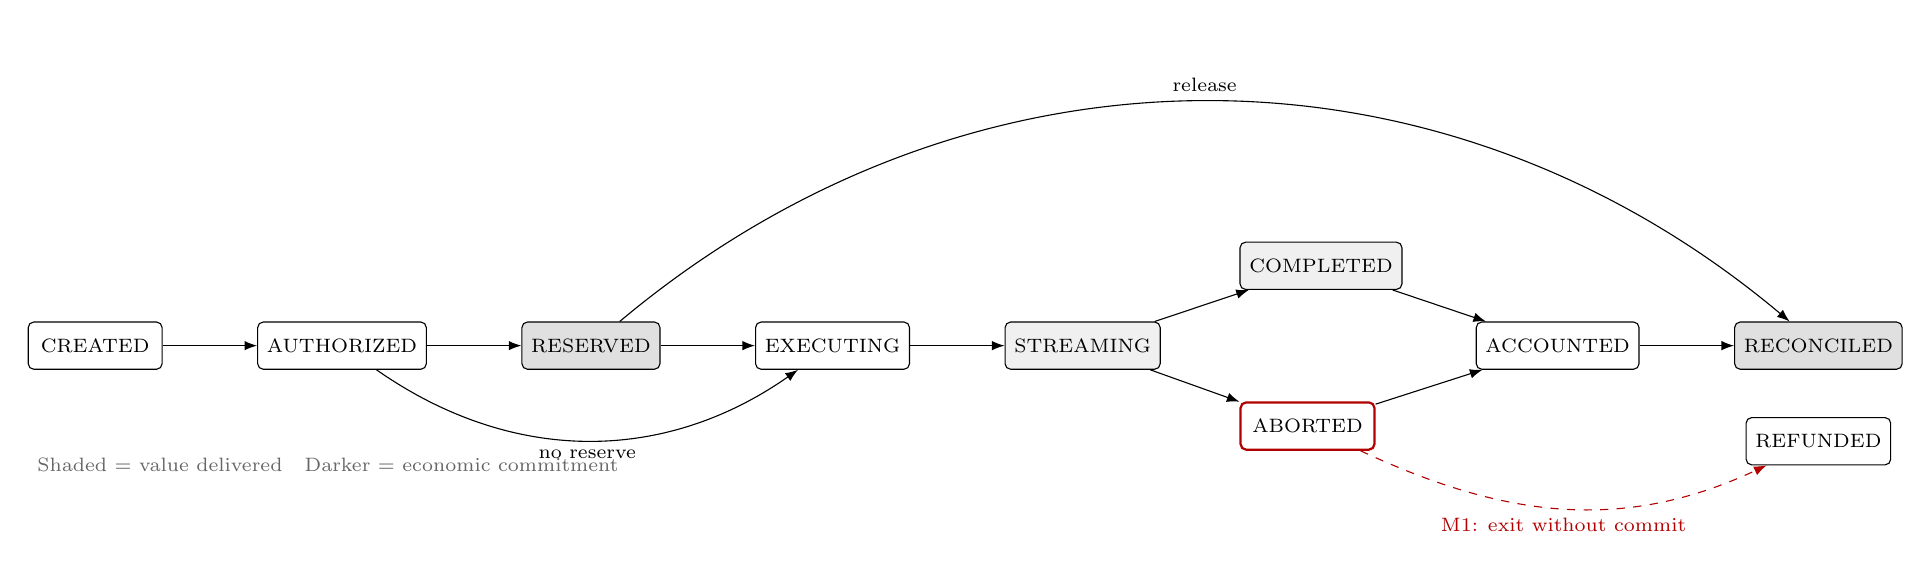
\begin{tikzpicture}[
  node distance=8mm and 12mm,
  every node/.style={font=\scriptsize},
  st/.style={draw, rounded corners=2pt, minimum height=6mm, minimum width=17mm, align=center},
  val/.style={st, fill=black!6},
  com/.style={st, fill=black!12},
  bad/.style={st, draw=red!70!black, thick},
  ->/.default=,
  arr/.style={-{Latex[length=1.6mm]}, thin},
  barr/.style={-{Latex[length=1.6mm]}, thin, red!70!black, dashed},
]
\node[st] (created) {CREATED};
\node[st, right=of created] (auth) {AUTHORIZED};
\node[com, right=of auth] (res) {RESERVED};
\node[st, right=of res] (exec) {EXECUTING};
\node[val, right=of exec] (stream) {STREAMING};
\node[val, above right=4mm and 10mm of stream] (comp) {COMPLETED};
\node[bad, below right=4mm and 10mm of stream] (abort) {ABORTED};
\node[st, right=14mm of stream, xshift=26mm] (acc) {ACCOUNTED};
\node[com, right=of acc] (rec) {RECONCILED};
\node[st, below=6mm of rec] (ref) {REFUNDED};
\draw[arr] (created) -- (auth);
\draw[arr] (auth) -- (res);
\draw[arr] (res) -- (exec);
\draw[arr] (auth) to[out=-35,in=-145] node[below,pos=.5]{no reserve} (exec);
\draw[arr] (exec) -- (stream);
\draw[arr] (stream) -- (comp);
\draw[arr] (stream) -- (abort);
\draw[arr] (comp) -- (acc);
\draw[arr] (abort) -- (acc);
\draw[arr] (acc) -- (rec);
\draw[barr] (abort) to[out=-25,in=-155] node[below,pos=.5]{\color{red!70!black}M1: exit without commit} (ref);
\draw[arr] (res) to[out=40,in=140] node[above,pos=.5]{release} (rec);
\node[align=left, anchor=north west] at ($(created.south west)+(0,-10mm)$) {%
  \color{black!60}Shaded = value delivered\quad Darker = economic commitment};
\end{tikzpicture}%
}
\caption{Request lifecycle. Value exposure begins at the first delivered token
(STREAMING); economic commitment is final only at RECONCILED. The interval between them
is the exposure window that M1 exploits. B0 corrupts the AUTHORIZED $\rightarrow$
RESERVED transition (non-atomic); M2 corrupts the data used at ACCOUNTED.}
\Description[State diagram of a metered request lifecycle]{A left-to-right state diagram
starts at CREATED and proceeds through AUTHORIZED, optionally RESERVED, EXECUTING, and
STREAMING. STREAMING branches to COMPLETED or ABORTED; both normally lead to ACCOUNTED and
then RECONCILED. A dashed red path shows the M1 failure, in which an aborted request exits
to REFUNDED without a committed charge. Shading marks states where value has been delivered
and darker shading marks economic commitment.}
\label{fig:statemachine}
\end{figure}

\subsection{Formal model}
For a request $r$ let $U_{\text{true}}(r)$ be the usage actually produced,
$U_{\text{bill}}(r)$ the usage billed, and $P(\cdot)$ the exact-decimal pricing function,
so that $C(r) = P(U_{\text{true}}(r))$ is the true cost. $V(r)$, $\mathrm{Res}(r)$,
$D(r)$, $F(r)$, and $N(r) = D(r) - F(r)$ are as defined in Section~\ref{sec:threat}
(Equations~\ref{eq:integrity}--\ref{eq:refund}). At trial level the harness independently
verifies conservation, $\sum_{r \in T} N(r) = B_{\text{initial}} - B_{\text{final}}$, and
fails the build on any divergence.

\subsection{Mechanism localization}
\paragraph{B0 (synchronization)}
The baseline implementation manifests as follows: if two concurrent requests read the
same authorization state $B$ and both commit a decrement derived from it, one decrement
is lost, $\sum_i N(r_i) < \sum_i V(r_i)$. This particular manifestation requires two or
more overlapping transactions, which is why the baseline leaks nothing at concurrency 1.
The general failure condition is broader than this trigger, however: the defect occurs
whenever authorization observes a state that does not yet reflect the economic
commitments generated by other authorized requests. Concurrent overlap is one way to
create that condition; Section~\ref{sec:b0revised} shows that deferred settlement creates
the same condition under strictly sequential arrivals, with no overlap at all. We
therefore distinguish, throughout this paper, the \emph{baseline trigger} (concurrent
overlap, in this implementation) from the \emph{general security condition}
(authorization not atomically coupled to economic commitment on the authorizing path).

\paragraph{M1 (commitment timing)}
If $V(r) > 0$ in STREAMING but the exit path taken (ABORTED) does not reach RECONCILED
with $N(r) \ge V(r)$, then $\mathrm{Leak}(r) = V(r) > 0$. The defect is in the transition
graph, not in a shared resource: it is a per-request lifecycle property, and
Section~\ref{sec:m1} confirms empirically that it does not depend on concurrency in the
tested architecture.

\paragraph{M2 (usage authority)}
If the billing basis is client-controlled, $U_{\text{bill}} = T(U_{\text{true}})$ for an
attacker transformation $T$, then $\mathrm{Leak}(r) = P(U_{\text{true}}) -
P(T(U_{\text{true}})) > 0$ whenever $P \circ T < P$. Authority is a per-request
data-provenance property; Section~\ref{sec:m2} shows this is analytically independent of
concurrency because the billed amount never reads shared mutable state.

\begin{table}[t]
\centering
\caption{Structural distinction between the three mechanisms: what is defective, what
triggers the baseline manifestation we implemented, and what closes it. ``Trigger'' is
implementation-specific; the general condition (final column of Table~\ref{tab:practical})
is what actually matters and is not concurrency-specific for any of the three.}
\label{tab:structural}
\resizebox{\linewidth}{!}{%
\renewcommand{\arraystretch}{0.92}%
\begin{tabular}{llll}
\toprule
Mechanism & Defective element & Baseline trigger (this implementation) & Closed by \\
\midrule
B0 & transition atomicity & overlapping requests (concurrency $\ge 2$); deferred settlement also suffices (Sec.~\ref{sec:b0revised}) & authorization atomically coupled to commitment on the authorizing path \\
M1 & transition graph (abort path) & any single abort, no concurrency needed & abort-inclusive finalization \\
M2 & data authority at ACCOUNTED & any single request with a client-controlled billing basis, no concurrency needed & server-authoritative recount \\
\bottomrule
\end{tabular}%
}
\end{table}

Read architecturally, the three mechanisms sit at three different kinds of boundary. B0
concerns state ownership on the authorization path: which component reads the balance,
and whether that read and the economic commitment are one atomic step. M1 concerns the
settlement path: whether every terminal path of the request lifecycle reaches a committed
accounting event. M2 concerns data authority: which representation of usage the billing
function reads. Solvency and accounting integrity are separated in M1 because different
steps of the lifecycle own them, reservation before execution and finalization on every
exit path.

Section~\ref{sec:results} confirms this prediction empirically: the B0 manifestation we
implemented requires concurrency; M1 and M2 per-request leakage does not.

\section{Architectural Taxonomy}
\label{sec:taxonomy}
The three dimensions just distinguished architecturally are also experimentally
distinguishable, not merely conceptual: B0 is a non-atomic authorize-then-decrement on
shared credit state, a known baseline used to validate the measurement rig and supply a
generic reference point, while M1 and M2 remain the lifecycle- and authority-sensitive
dimensions of Section~\ref{sec:statemodel}.

\subsection{On LLM specificity}
We do not claim these mechanisms are possible only in LLM systems. Streaming responses,
trusting client-supplied values, and racing a counter all occur elsewhere. What is
specific to LLM inference is that one request combines, at a single metering boundary:
progressive value delivery; usage that is generated at runtime and therefore unknown at
authorization time; multi-category token vectors; tokenizer- and provider-dependent usage
semantics; pricing functions defined over those categories; and asynchronous settlement.
It is the combination we systematize, not the individual pieces.

The three dimensions generalize to different degrees, stated rather than blurred. B0 is
fully generic: a shared-counter race that behaves the same in any metered service, and
the revised condition of Section~\ref{sec:b0revised} -- that authorization be atomically
coupled to economic commitment on the authorizing path -- is a statement about
distributed accounting state with no reference to inference at all. M1 generalizes to any
service that delivers value progressively over a long-running request, streamed media and
batch jobs included, and is interesting exactly where a terminal path can bypass the
accounting event. M2 is the narrowest: it needs a billed quantity that is
runtime-produced, multi-category, and priced by a category-sensitive function, currently
most visible in LLM APIs but not unique to them.

The boundary studied here is the usage-metering and accounting subsystem of a
network-accessible serving system: an authorization path, a settlement path, and an
accounting event lifecycle, with state ownership divided among the gateway, the
accounting store, and, in the asynchronous family, an event pipeline, and a
data-authority decision at ACCOUNTED about which representation of usage the billing
function reads. We do not study the behavior, robustness, or output safety of the
language model itself.

\section{System and Experimental Methodology}
\label{sec:method}
The experiments validate the architectural behavior and engineering claims of the
preceding sections -- not a user study, industrial evaluation, or field deployment -- and
the study deliberately trades realism for control and precision \citep{abc}. The testbed is a FastAPI gateway over PostgreSQL 16 in READ COMMITTED and Redis 7,
running under Docker Compose on one commodity host with 16 logical CPUs and 16\,GB of
RAM. Money is exact decimal throughout. Five M1 architectures and six M2 architectures
sit behind common interfaces, so experiments compare semantics rather than unrelated
code. The default generator is deterministic, which is what makes the accounting
arithmetic exact; real tokenizers run on the recount path, and
Section~\ref{sec:generality} replaces the generator entirely with third-party serving
code.

Pricing is category-wise over three tiers. Leakage \emph{efficiency}, the fraction of
true value evaded, is the headline metric because it is invariant under uniform price
scaling; absolute dollar figures are labeled as scenario values. The sweeps are: B0
concurrency $\{1,2,5,10,20,30,50\}$ with 30 repetitions; M1 across architecture, abort
position, and concurrency $\{1,5,20,50,100\}$; M2 across architecture, manipulation, and
concurrency. Request volume is held constant across concurrency levels, so that volume
cannot masquerade as vulnerability.

\subsection{Integrity gates}
Every summarizer recomputes each record's leak from primitives, checks invariant-flag
consistency, and verifies ledger conservation $\sum_r N(r) = B_{\mathrm{init}} -
B_{\mathrm{final}}$ without trusting the application's own bookkeeping. A violation fails
the build. The gates are validated adversarially, not assumed: corrupting a leak value,
debit, served flag, balance, or invariant flag, and deleting a ledger row, must each be
detected -- and all twelve injections were. The metamorphic suite also caught
one of our own unjustified assumptions. We had asserted that leakage efficiency is
invariant across price tiers; it is, but only under uniform scaling, not under a
structural change to the price ratios. We corrected the property rather than suppress the
failure.

\subsection{Independent verification}
The strongest M2 defense is re-implemented in a module that shares no code path with the
gateway, and the two agree on all cross-validated cells (42 M2, 16 M1, 2 B0). A separate
audit re-derives every reported quantity from raw data using code that imports nothing
from the project, and reports zero discrepancies across 4{,}800 M2 records, 2{,}400 M1
records, and 420 B0 trials. The independent checker initially reported three
disagreements. They were definitional, not defects: the checker aggregated under-payment
only, the gateway the signed billing delta, and under flat-total pricing an honest client
is systematically overcharged, so the two aggregates legitimately differ. Both are now
reported, and the security property uses under-payment.

\subsection{Statistics}
All statistics come from a standalone script using SciPy \citep{scipy} and statsmodels
\citep{statsmodels}, writing a
single output file that the paper cites. Many conditions here are deterministic by
construction and have exactly zero variance. For those we report the constant and the
complete separation rather than a $p$-value, and reserve nonparametric tests and
bootstrap intervals \citep{efron} for quantities that genuinely vary, in line with common
guidance for the statistical analysis of randomized experiments in software engineering
\citep{arcuri}.

\subsection{Reproducibility}
The artifact is archived with a DOI, with raw data and reproduction scripts released
alongside it. Repeatability of computer-systems research is known to be weak
\citep{collberg}, and repeatability, reproducibility, and corroboration are distinct
goals \citep{feitelson}; we address the first two by releasing code and raw data, not the
third. The release is consistent in spirit with the FAIR principles for research data
\citep{fair}.

For this upgrade, a second independent raw-data auditor imported no measurement-producing
module and recomputed 2{,}400 M1 records, 4{,}800 M2 records, and 420 B0 trials with zero
arithmetic, duplicate-ID, or required-field discrepancies. Its preregistered E2 extension
repriced 3{,}120 frozen M2 records under three pricing bases (9{,}360 record--basis cells):
server-authoritative architectures had zero positive-leak cells and zero pricing-field
dependency violations. The maximum stored real-inference recount fraction independently
recomputed to 0.023693\%.

\section{Formal Verification}
\label{sec:formal}
Measurement shows a defect occurs on the schedules our harness produced; it cannot show a
defended architecture is safe on schedules it did not produce. We therefore encode the
lifecycle of Section~\ref{sec:statemodel} in TLA+ \citep{tla} and check it exhaustively
with TLC 2.19 \citep{tlc}. In software-verification terms, the specification is an
executable architectural model against which each configuration's safety properties are
checked; it verifies the model, not the implementation.

\subsection{Model}
One specification covers all three dimensions, with each dimension as a Boolean constant,
so that the safe and unsafe architectures are the same state machine under different
constants, exactly how the testbed implements them behind one interface. The constants
are \texttt{AtomicDebit} for B0, \texttt{Reserves} and \texttt{AbortSafe} for M1, and
\texttt{ServerAuthority} for M2. A fifth constant, \texttt{ClientMayAbort}, is a workload
switch rather than an architecture property; disabling it in the B0 configurations keeps
the synchronization counterexample free of commitment-timing noise, mirroring how the
experiments hold the other dimensions at their safe setting.

Four invariants are checked, each the formal counterpart of a gate the summarizers
already apply to every record: \textsc{AccountingIntegrity} ($V(r) \le N(r)$ for terminal
$r$), \textsc{Solvency} ($\mathrm{balance} \ge 0$), \textsc{LedgerConservation} (once all
requests are terminal, $B_{\mathrm{init}} - B_{\mathrm{final}} = \sum_r N(r)$), and
\textsc{RefundBounded}, which is Equation~(\ref{eq:refund}). Solvency is checked
separately from accounting integrity; collapsing them would destroy the distinction the
ablation exists to establish.

\subsection{Method}
Each invariant is checked in its own TLC run. TLC halts at the first violation it finds,
so checking jointly would hide the fact that an M2 architecture breaks two of them. The
result is a full configuration $\times$ invariant matrix (Table~\ref{tab:formalmatrix}):
ten configurations and four invariants give 40 independent runs over 27{,}526 distinct
states. Every expected outcome is declared in the checking script before the run, which exits
non-zero on any disagreement; all 40 matched. Runs
use a single worker deliberately: with parallel workers, a run that halts at a
counterexample explores a nondeterministic number of states, and the totals drifted
between runs.

\begin{table}[t]
\centering
\caption{TLC model-checking results across ten architecture configurations and four
invariants. All 40 outcomes matched the expectation declared before the run.}
\label{tab:formalmatrix}
\resizebox{\linewidth}{!}{%
\renewcommand{\arraystretch}{0.92}%
\begin{tabular}{lllll}
\toprule
Configuration & Accounting integrity & Solvency & Ledger conservation & Refund bounded \\
\midrule
b0 vulnerable & holds & holds & VIOLATED & holds \\
b0 hardened & holds & holds & holds & holds \\
m1 post completion & VIOLATED & holds & holds & holds \\
m1 reserve refund on abort & VIOLATED & holds & holds & VIOLATED \\
m1 no reserve settle & holds & VIOLATED & holds & holds \\
m1 reserve reconcile & holds & holds & holds & holds \\
m2 client & VIOLATED & holds & holds & VIOLATED \\
m2 server recount & holds & holds & holds & holds \\
all defenses & holds & holds & holds & holds \\
all defenses 3req & holds & holds & holds & holds \\
\bottomrule
\end{tabular}}
\end{table}

\subsection{Counterexamples}
TLC returns a shortest counterexample for each unsafe configuration, and each reproduces
the mechanism we measured. For B0, the 21-step trace is the lost update exactly: both
requests read the same balance, both write an absolute value derived from that stale
read, and both then deliver and are charged. Which invariant fails is the interesting
part. Accounting integrity and the refund bound both hold, because every individual
record is internally consistent; what breaks is conservation of the shared balance. That
is why a per-record audit cannot detect B0 while a conservation check can.

For M1, the model checks all four combinations of reservation and abort-safe
finalization, not just the two the implementation ships. Reservation alone yields
solvency and violates integrity. Abort-safe finalization alone yields integrity and
drives the balance to $-1$. Only the conjunction satisfies both. The orthogonality claim
is therefore established by exhaustive exploration rather than by the two architectures
we happened to build.

For M2, the client-authoritative architecture violates accounting integrity and also the
refund bound: with a reservation in place, under-billing surfaces as an over-refund. That
the same defect appears in two independent invariants is a consequence of the model, not
something we set out to show, visible only because the invariants are checked
separately. Enabling server authority restores all four invariants
against the same lying client; the declared value simply stops being read.

The three defenses also compose. With contention, aborts, and a lying client all enabled,
no invariant is violated on any reachable state, at two and at three concurrent requests.

\subsection{Evidence labels and their limits}
We use three labels and do not interchange them. \emph{Model-checked} means TLC explored
the reachable state space exhaustively under a stated configuration. \emph{Formally
argued} means stated over the accounting model and reasoned about by hand.
\emph{Empirically verified} means measured and independently recomputed. Nothing weaker
than the first is ever described as proved.

Nothing here shows a production implementation is safe: the model abstracts away the
database, network, partial failure, asynchronous reconciliation, multi-category pricing,
and tokenizer disagreement, and is finite, at two to three requests with unit pricing;
only safety properties are checked, not liveness. \textbf{We
do not provide a mechanized refinement proof from the abstract specification to the
implementation}; the correspondence between the two is an argument supported by
case-by-case agreement between formal and empirical outcomes, not more.

\subsection{Validating the specification}
Declaring expectations before running earned its keep immediately. Our first
specification treated a reservation as a hold and set the committed debit equal to the
charge at settlement, so $N = D - F$ fell below the delivered value and TLC rejected the
safe configurations. The model was wrong, not the paper: in a reserve-and-reconcile
architecture the reservation \emph{is} the committed debit, and the refund returns its
unused part. Correcting the settlement semantics made the safe configurations verify; we record the
failure because a formal model edited until it agrees with the paper is worth nothing.

\subsection{A second model: the asynchronous-settlement race}
\label{sec:asyncformal}
The specification above assumes strongly consistent accounting state and is silent on
the mechanism behind Section~\ref{sec:b0revised}: deferred settlement, not concurrency,
separating authorization from commitment. We built a second, separate TLA+
specification, \texttt{AsyncSettlementTOCTOU.tla}, rather than extending the first,
because the two mechanisms are different in kind. It is a causal-ordering model, not a
timed one: a request moves through \textsc{created}
$\to$ \textsc{admitted}/\textsc{rejected} $\to$ \textsc{settlement\_pending} $\to$
\textsc{settled} (or \textsc{released}), and interleavings are ordered by happens-before,
not by milliseconds, matching the T1--T7 instrumentation's own finding that the
authorization step is a plain read and only settlement ever writes the balance.

We checked it with TLC at six preregistered $(N,k)$ points: $(3,1)$, $(4,1)$, $(4,2)$,
$(5,2)$, $(6,2)$, and $(6,3)$. The $(6,2)$ point matches the primary B0-async workload,
and $(4,2)$ matches a second tested empirical configuration; the remaining four are a
preregistered bounded extension. In the vulnerable configuration, \textsc{Solvency} is
violated at all six points; TLC's shortest
counterexample at $(6,2)$ needs only three staggered, non-simultaneous admissions against
a two-unit budget. \textsc{AccountingIntegrity} and \textsc{LedgerConservation} hold at
all six bounded points (the $(6,2)$ holding runs re-checked in isolation explored 91{,}921
generated and 22{,}521 distinct states, with no violation). In the atomic configuration
all three invariants hold at all six points. Across 36 single-invariant runs, all outcomes
matched the preregistered expectations; sums across repeated invariant runs were 480{,}565
generated and 116{,}920 distinct states.

This contrasts usefully with Table~\ref{tab:formalmatrix} rather than repeating it: the
synchronous model's vulnerable B0 configuration violates \textsc{LedgerConservation} and
holds \textsc{Solvency}, the signature of a lost update; this model's vulnerable
configuration violates \textsc{Solvency} and holds \textsc{LedgerConservation}, the
signature of an admission race with no lost write at all. Two mechanistically distinct
races leave different invariant fingerprints, itself a cross-check between the two
specifications rather than noise to explain away.

The same evidence labels and limits apply as in Section~\ref{sec:formal}'s own account of
itself: this is \emph{model-checked}, exhaustively, at six finite $(N,k)$ points, over an
abstract, untimed model of the mechanism. It does not verify the implementation, a timed
or networked behavior, or anything beyond the six configurations checked, and it is the
formal counterpart of the empirical result in Section~\ref{sec:netsep}, not a substitute
for it.

\section{Empirical Results}
\label{sec:results}

\subsection{B0: synchronization}
The non-atomic check-then-decrement baseline leaks only when at least two requests
overlap; this is a property of the implemented trigger, and Section~\ref{sec:b0revised}
shows a different trigger for the same underlying condition. Mean leakage is \$0.000 at
concurrency 1, then \$0.099, \$2.871, and \$4.851 at concurrency 2, 30, and 50, growing
linearly at 0.099 per additional concurrent request with $R^2 = 1.0000$ and $p = 1.9
\times 10^{-50}$ (Figure~\ref{fig:b0}). The hardened atomic compare-and-decrement leaks
nothing at every level.
B0 is not a contribution; it validates the rig and supplies the contrast used below.
Section~\ref{sec:generality} revises the conclusion drawn from it.

\begin{figure}[t]
\centering
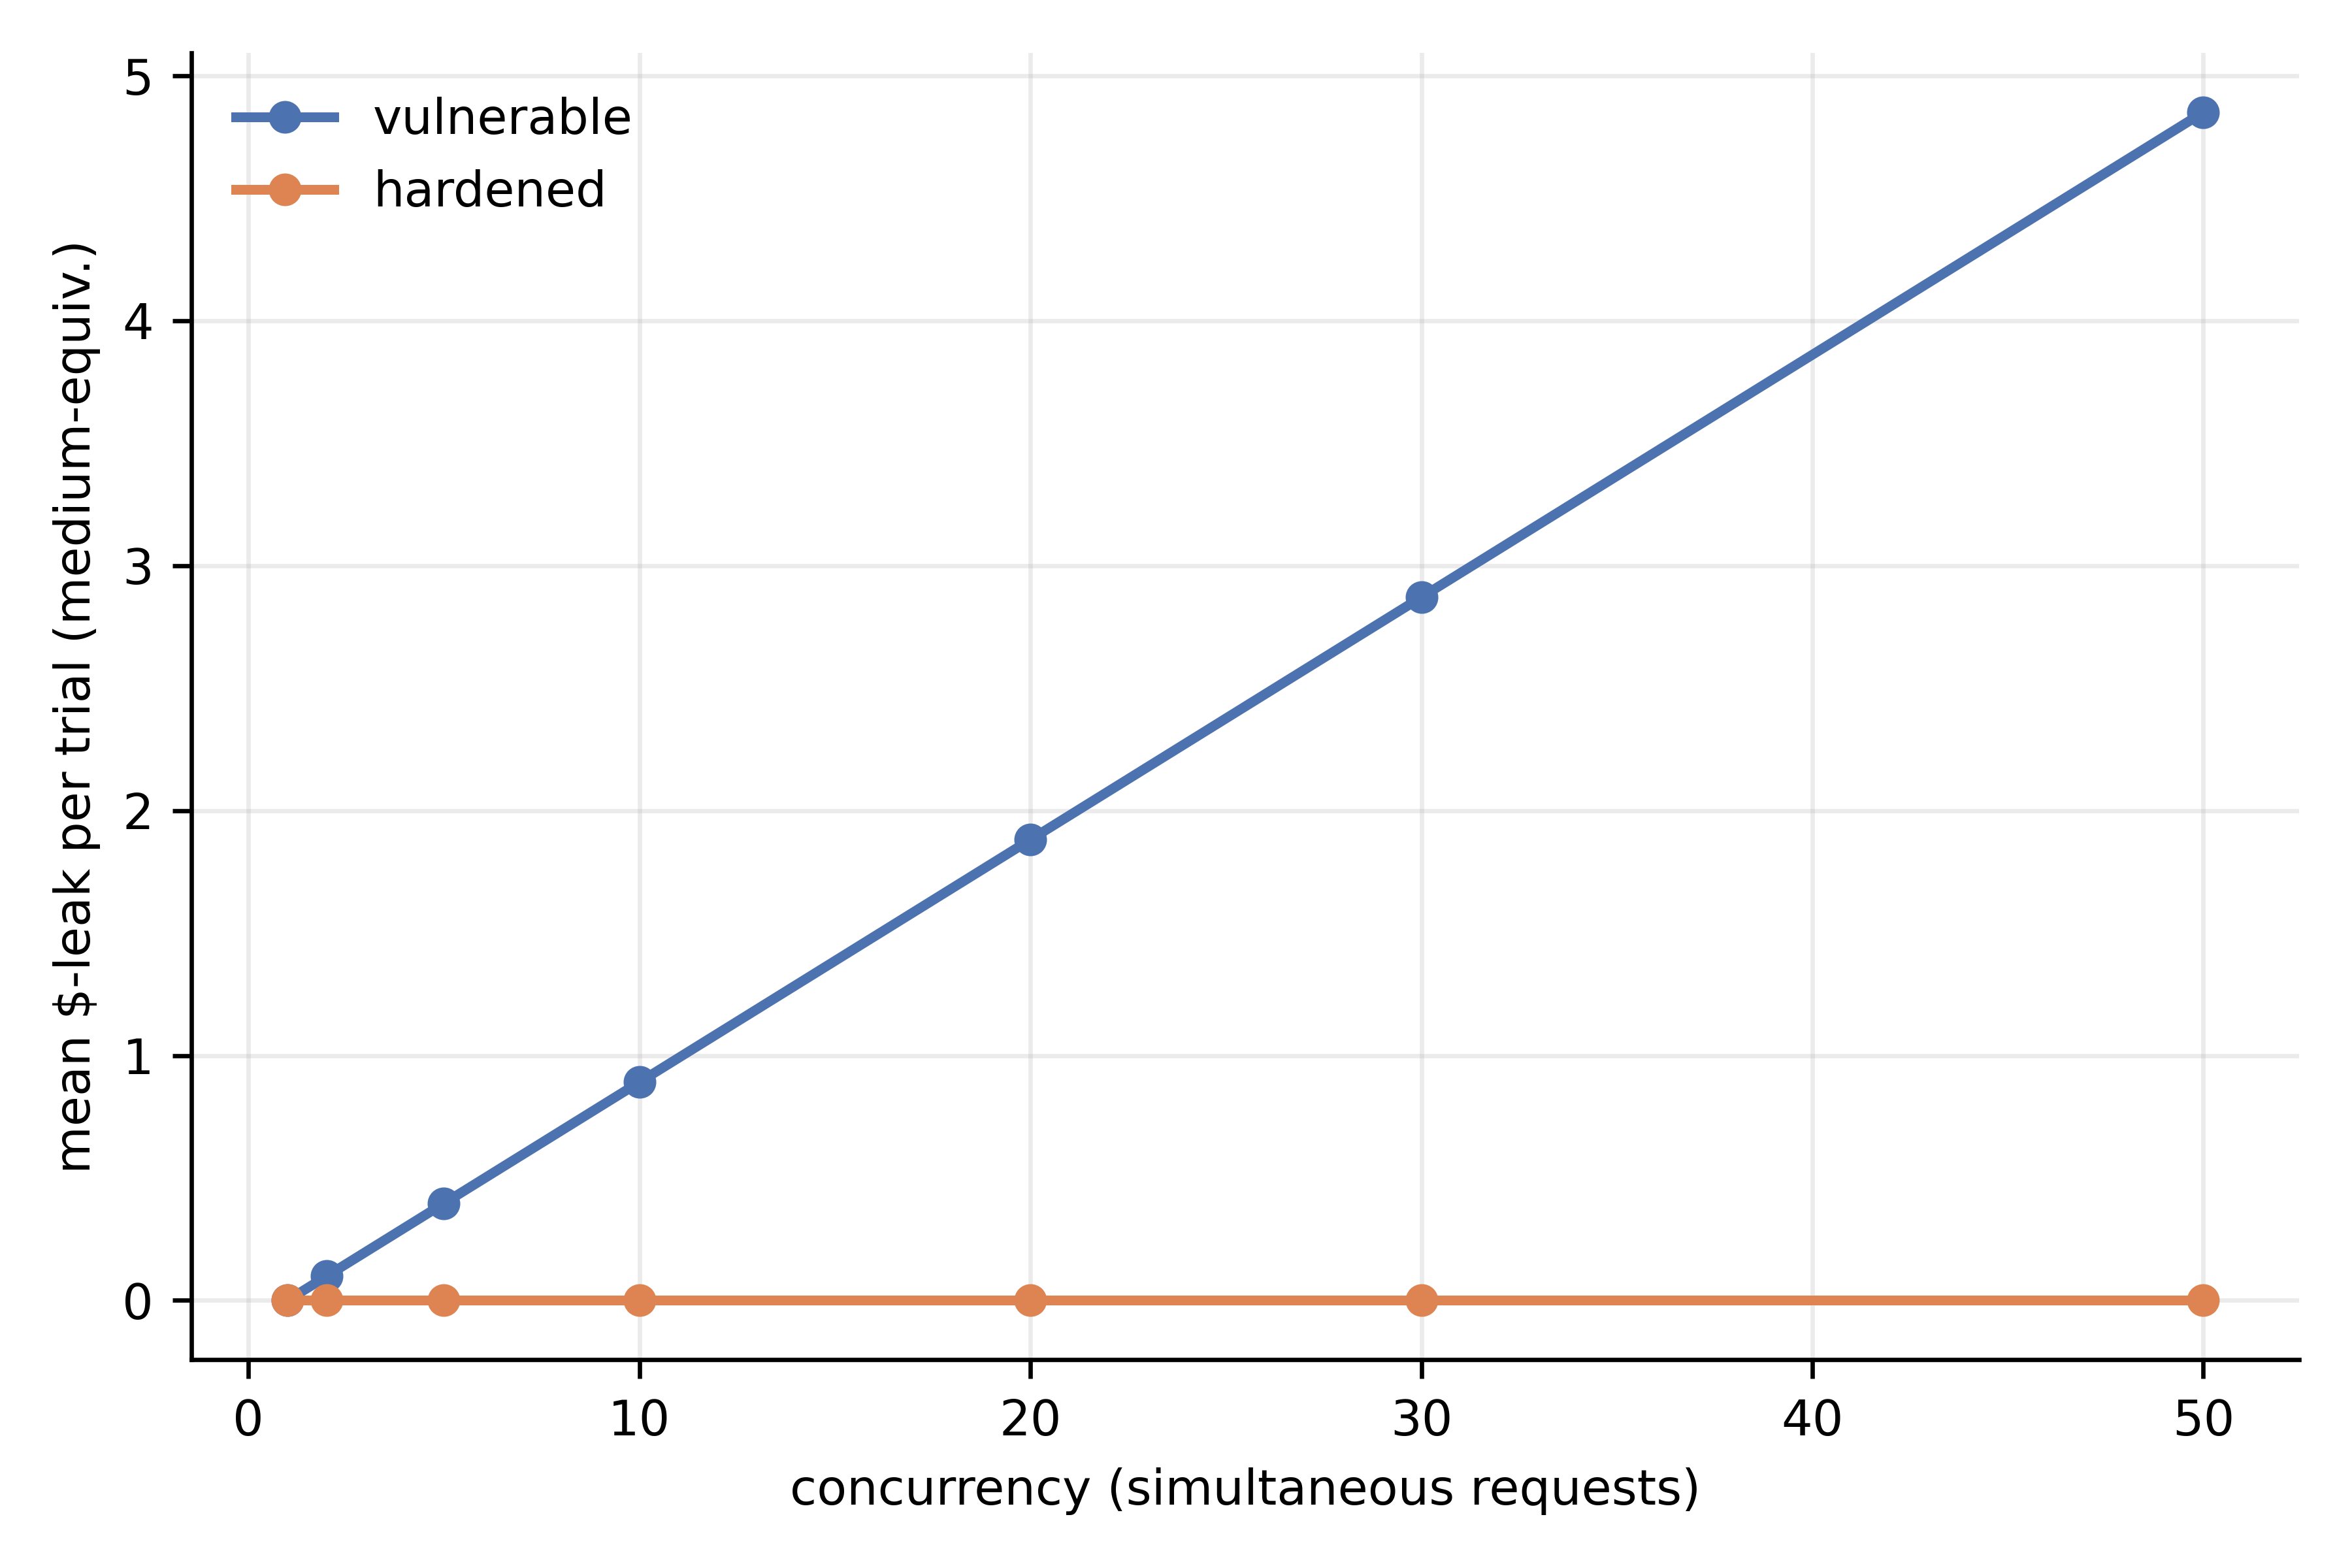
\includegraphics[width=\linewidth]{Figure_2.png}
\caption{B0 baseline: mean leakage per trial against concurrency, 30 repetitions per
cell, deterministic generator (linear fit in text). Section~\ref{sec:b0revised} shows
concurrency is not the essential ingredient: delayed settlement reproduces over-serving
with strictly sequential arrivals.}
\Description[Leakage rises with concurrency only in the vulnerable B0 implementation]{A
line chart compares vulnerable and hardened B0 implementations at concurrency levels from
1 to 50. The vulnerable line starts at zero for one request and rises approximately
linearly to 4.851 dollars at concurrency 50. The hardened line remains at zero for every
concurrency level.}
\label{fig:b0}
\end{figure}

\subsection{M1: commitment timing}
\label{sec:m1}
Leakage tracks the value delivered before the missing commit. It rises monotonically
with abort position and collapses to zero at completion, when the debit finally fires:
per request, \$0.0045 at roughly one token delivered, \$0.0285 at 25\%, \$0.0540 at 50\%,
\$0.0960 at 90\%, and \$0.0000 at completion (Figure~\ref{fig:m1}). Request-level attack
success is 1.00 at every abort position before completion. The two vulnerable
architectures, debit only after completion and refund the whole reservation on abort,
are economically identical.

\begin{figure}[t]
\centering
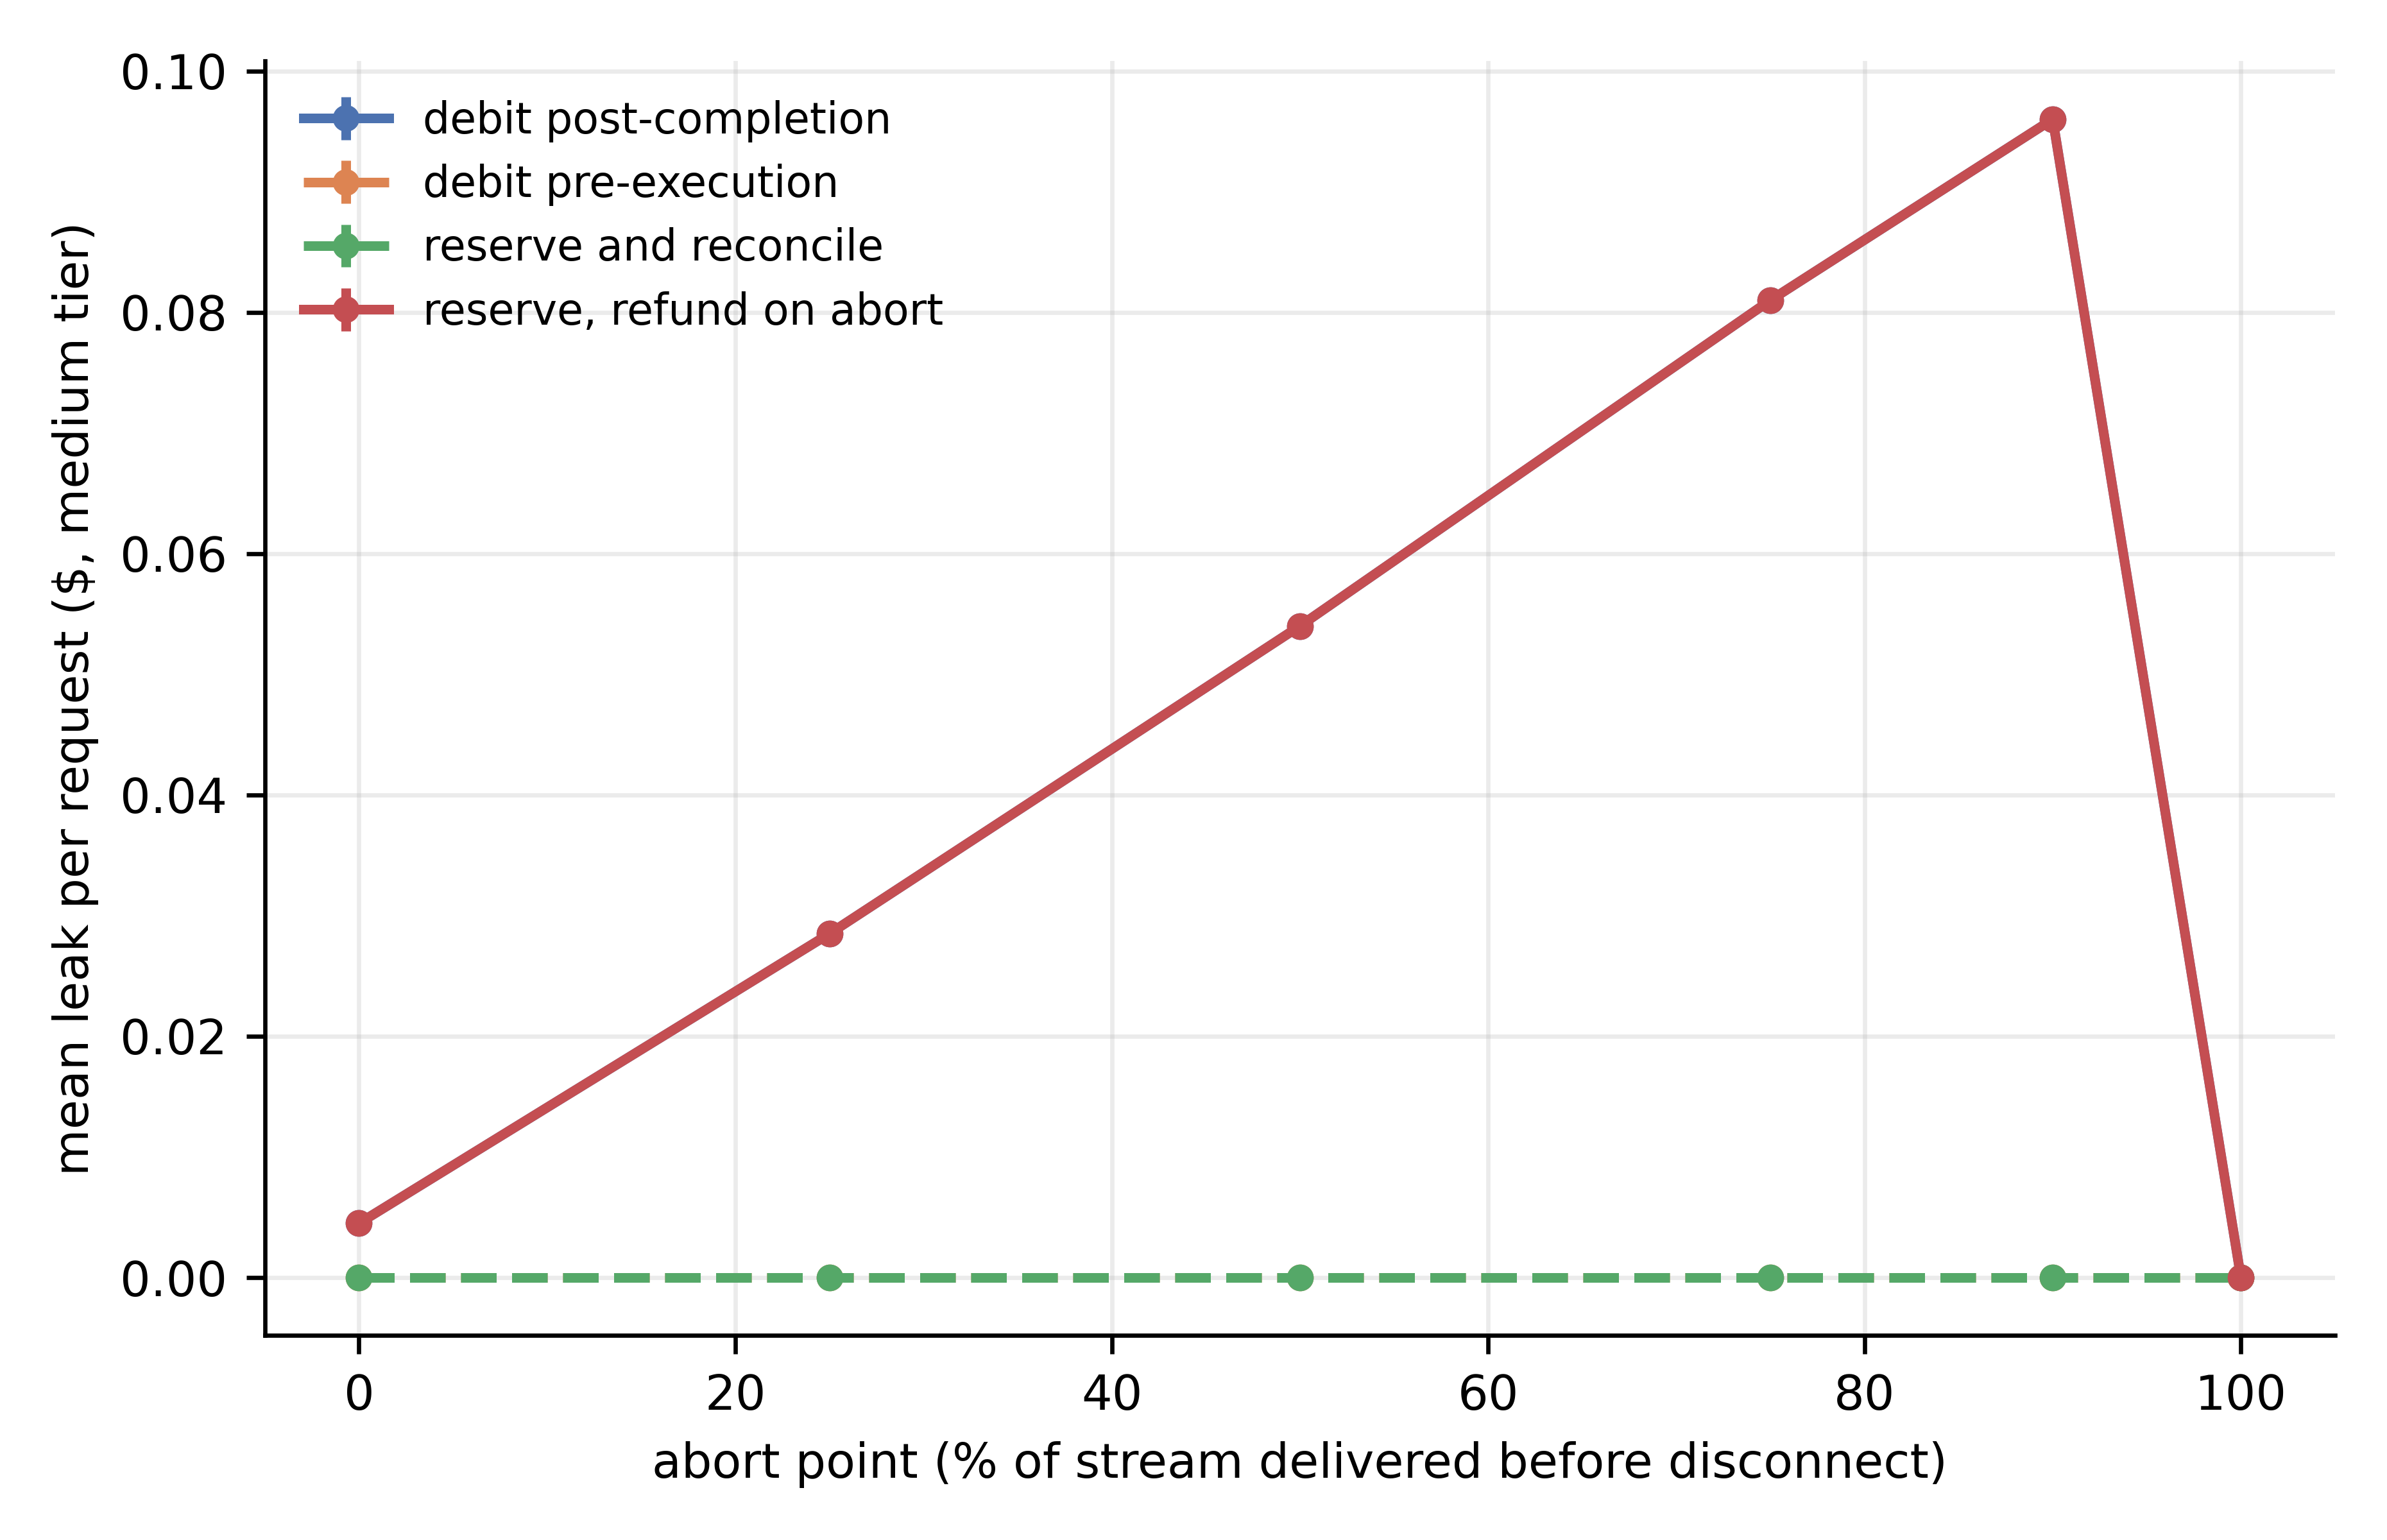
\includegraphics[width=\linewidth]{Figure_3.png}
\caption{M1 leakage (delivered value minus net committed debit) against abort position,
deterministic generator, concurrency 1, medium price tier, 20 requests per cell.
Vulnerable architectures peak just before the commit would have fired and collapse to
\$0 at completion; safe architectures stay at \$0 throughout. Error bars are within-cell
standard deviations, zero at this concurrency.}
\Description[Leakage depends on abort position for vulnerable M1 architectures]{A line
chart compares four settlement architectures as a stream progresses from zero to full
delivery. The debit-after-completion and reserve-then-refund-on-abort lines overlap,
rising from about 0.0045 dollars near the start to 0.096 dollars at 90 percent delivery,
then dropping to zero at completion. The debit-before-execution and
reserve-and-reconcile lines remain at zero throughout.}
\label{fig:m1}
\end{figure}

\subsubsection{Two orthogonal properties}
The ablation separates solvency from accounting finality. Given a budget for two requests
and six issued, the no-reserve-settle architecture preserves accounting integrity
(leakage is \$0.0000 at every abort position) yet serves all six and drives the balance
to $-\$0.32$. Conversely, the reserve-refund-on-abort architecture holds a reservation
and then refunds it away, failing both. Table~\ref{tab:m1orth} states the resulting
design rule; Section~\ref{sec:formal} establishes it exhaustively rather than by these
two examples.

\begin{table}[t]
\caption{M1 orthogonality. Each control secures one property; only the conjunction
secures both. All four cells are model-checked (Table~\ref{tab:formalmatrix}); the
diagonal cells are also measured.}
\label{tab:m1orth}
\centering
\begin{tabular}{lll}
\toprule
 & \multicolumn{2}{c}{Reservation} \\
\cmidrule(l){2-3}
Abort-safe finalization & No & Yes \\
\midrule
No & neither property & solvency only \\
Yes & integrity only & both \\
\bottomrule
\end{tabular}
\end{table}

\begin{figure}[t]
\centering
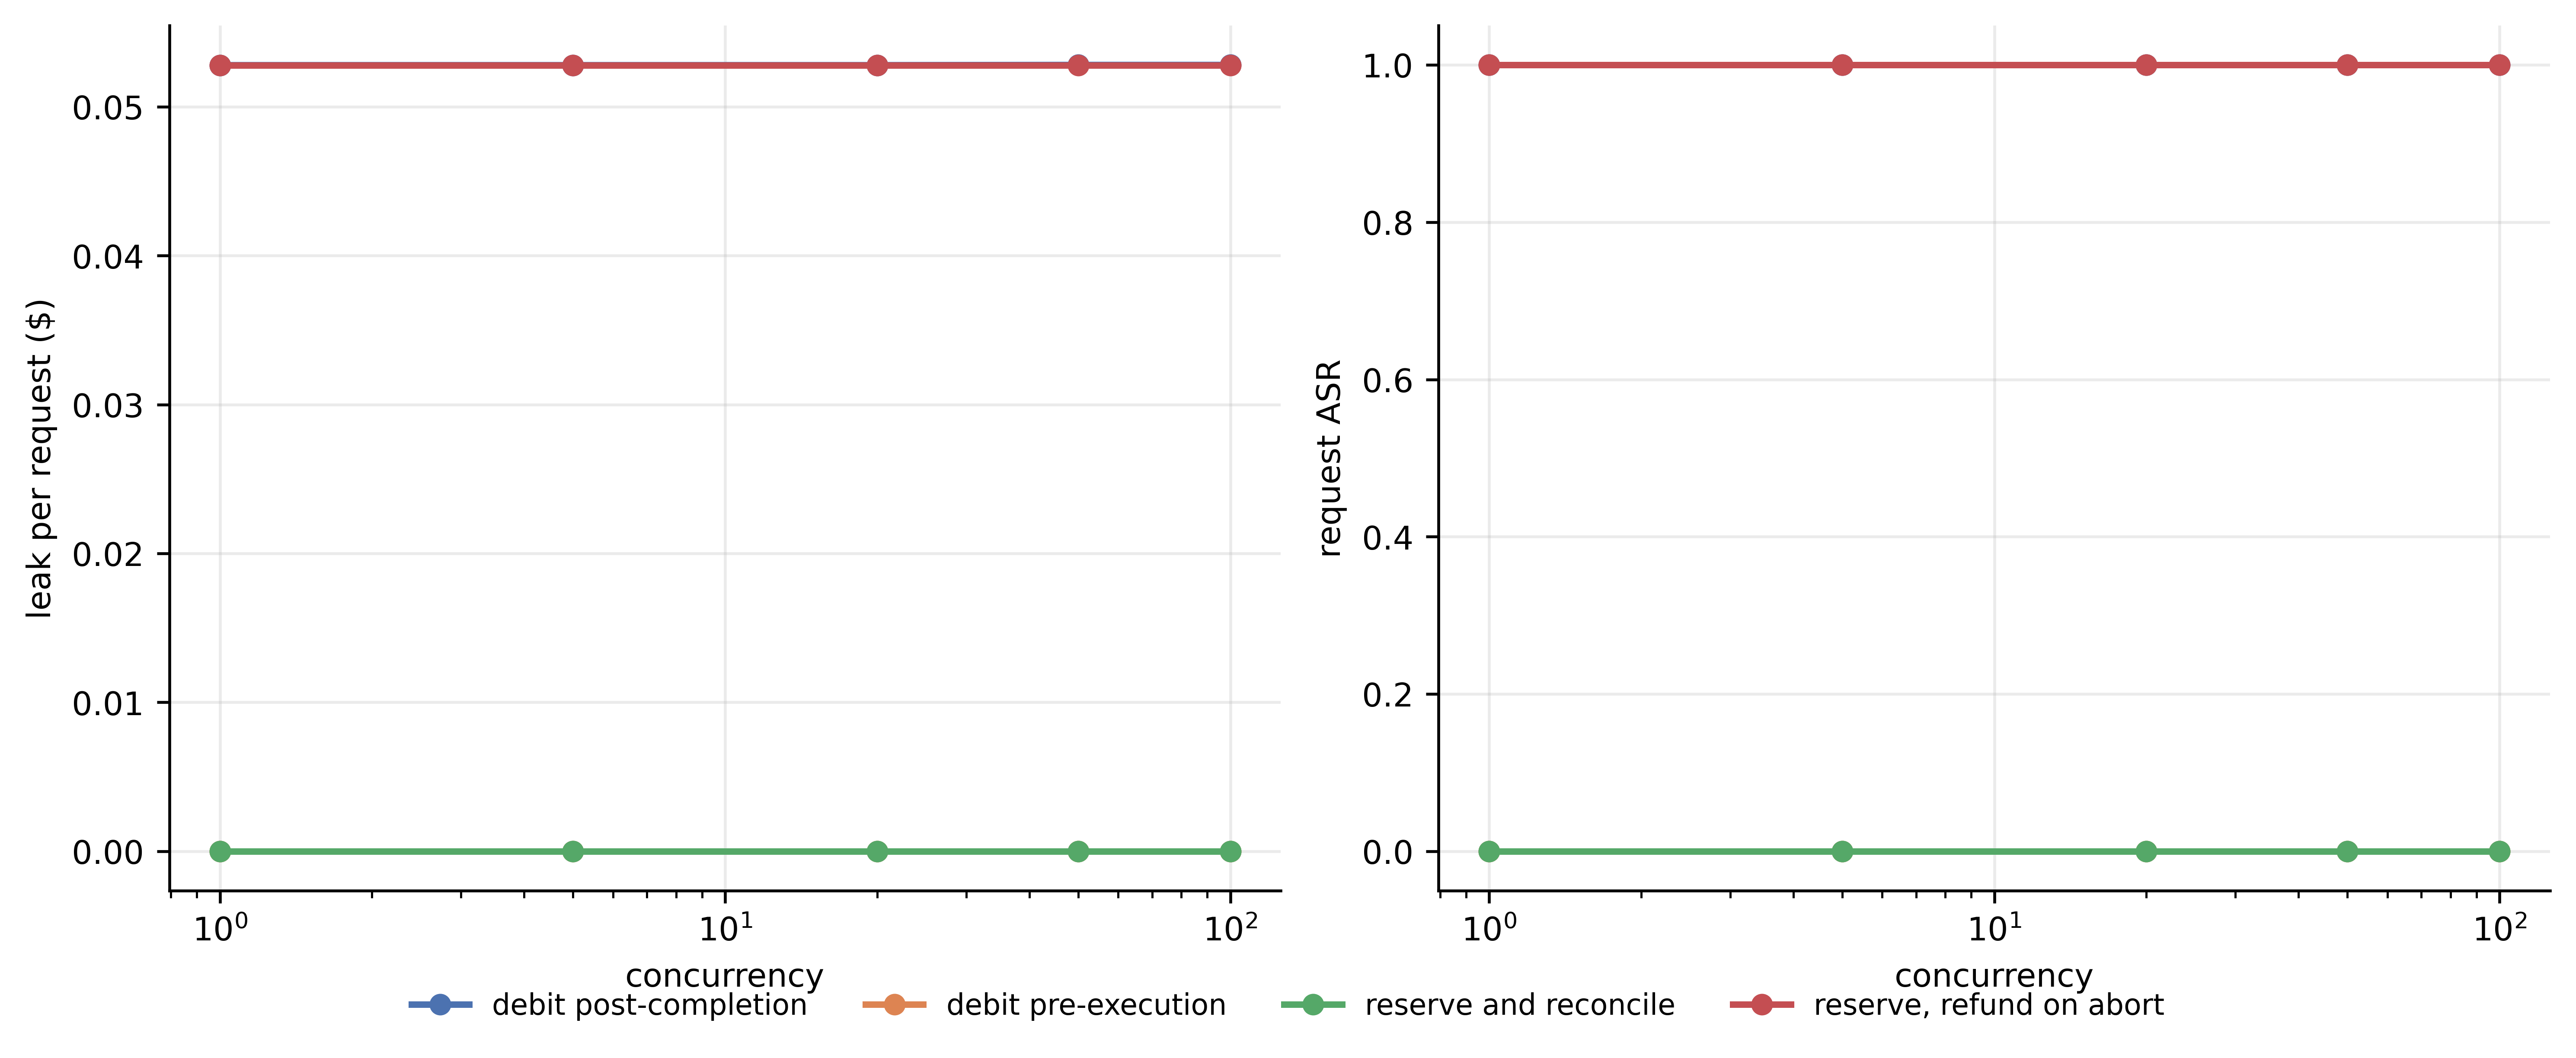
\includegraphics[width=\linewidth]{Figure_4.png}
\caption{M1 negative result: mean leakage per request and request-level attack success
against concurrency (1 to 100, log scale, volume fixed at 20 requests/cell). Both are
invariant across the range, the empirical basis for treating commitment timing as
per-request rather than contention-driven.}
\Description[M1 leakage and attack success are invariant to concurrency]{Two side-by-side
line charts use a logarithmic concurrency axis from 1 to 100. In the left chart, the two
vulnerable settlement architectures overlap at about 0.0528 dollars of leakage per
request while both safe architectures remain at zero. In the right chart, the vulnerable
architectures overlap at attack success rate 1.0 while the safe architectures remain at
zero. All lines are horizontal across the concurrency range.}
\label{fig:m1conc}
\end{figure}

\subsubsection{Concurrency is not the mechanism}
With request volume held constant, per-request leakage was unchanged across concurrency
levels 1 to 100: \$0.0528 per request at every level, identical to four decimal places,
with request-level attack success exactly 1.000 for vulnerable and 0.000 for safe
architectures (Figure~\ref{fig:m1conc}). The honest-client control leaked nothing
anywhere. We do not claim
invariance as a proven property of all systems under all loads; this is the measured
behavior of the tested architecture, and Section~\ref{sec:discussion} gives the
structural reason the model predicts it.

\subsection{M2: usage authority}
\label{sec:m2}
The M2 result is best read as a chain: true usage is produced by the model, turned into a
vector, stored, priced by a billing authority's choice of representation, and debited --
yet a system can compute and store correct usage while billing from a different,
attacker-influenced representation, with nothing in the chain flagging the discrepancy.

That is not hypothetical. The client-logged architecture performs an accurate
server-side recount, records it alongside the declared vector, and bills the declared
number. Against 90\% output under-reporting it leaks 58.3\% of delivered value in the
controlled setting, and 69.0\% against the real serving stack of
Section~\ref{sec:generality}. The manipulation is K0: a client can count the tokens it
received, so no privileged knowledge is required. Every server-authoritative
architecture (server-recount, hybrid-reconcile, and upstream) drove leakage
efficiency to 0.000 across all eight manipulations in the tested catalog
(Figure~\ref{fig:m2}).

Writing $U$ for the true usage vector, $P$ for the pricing function, and $T$ for the
attacker's transformation of declared usage, a manipulation pays off exactly when
\begin{equation}
P(T(U)) < P(U),
\label{eq:m2}
\end{equation}
that is, when the pricing basis reads the field $T$ changes. Section~\ref{sec:economics}
develops the consequences. The exploitable set is a property of the billing function, not
of attacker ingenuity.

M2's independence from concurrency is analytic rather than discovered. The billed amount
is a pure function of one request's declared usage, computed before any balance is read,
so no shared mutable state enters the billing decision and the leak of one request cannot
depend on what else is in flight. The concurrency sweep confirms the derivation and
serves as a check that the implementation contains no unintended shared-state dependency.
It passes, and we present it as a much weaker claim than B0's measured slope.

\begin{figure}[t]
\centering
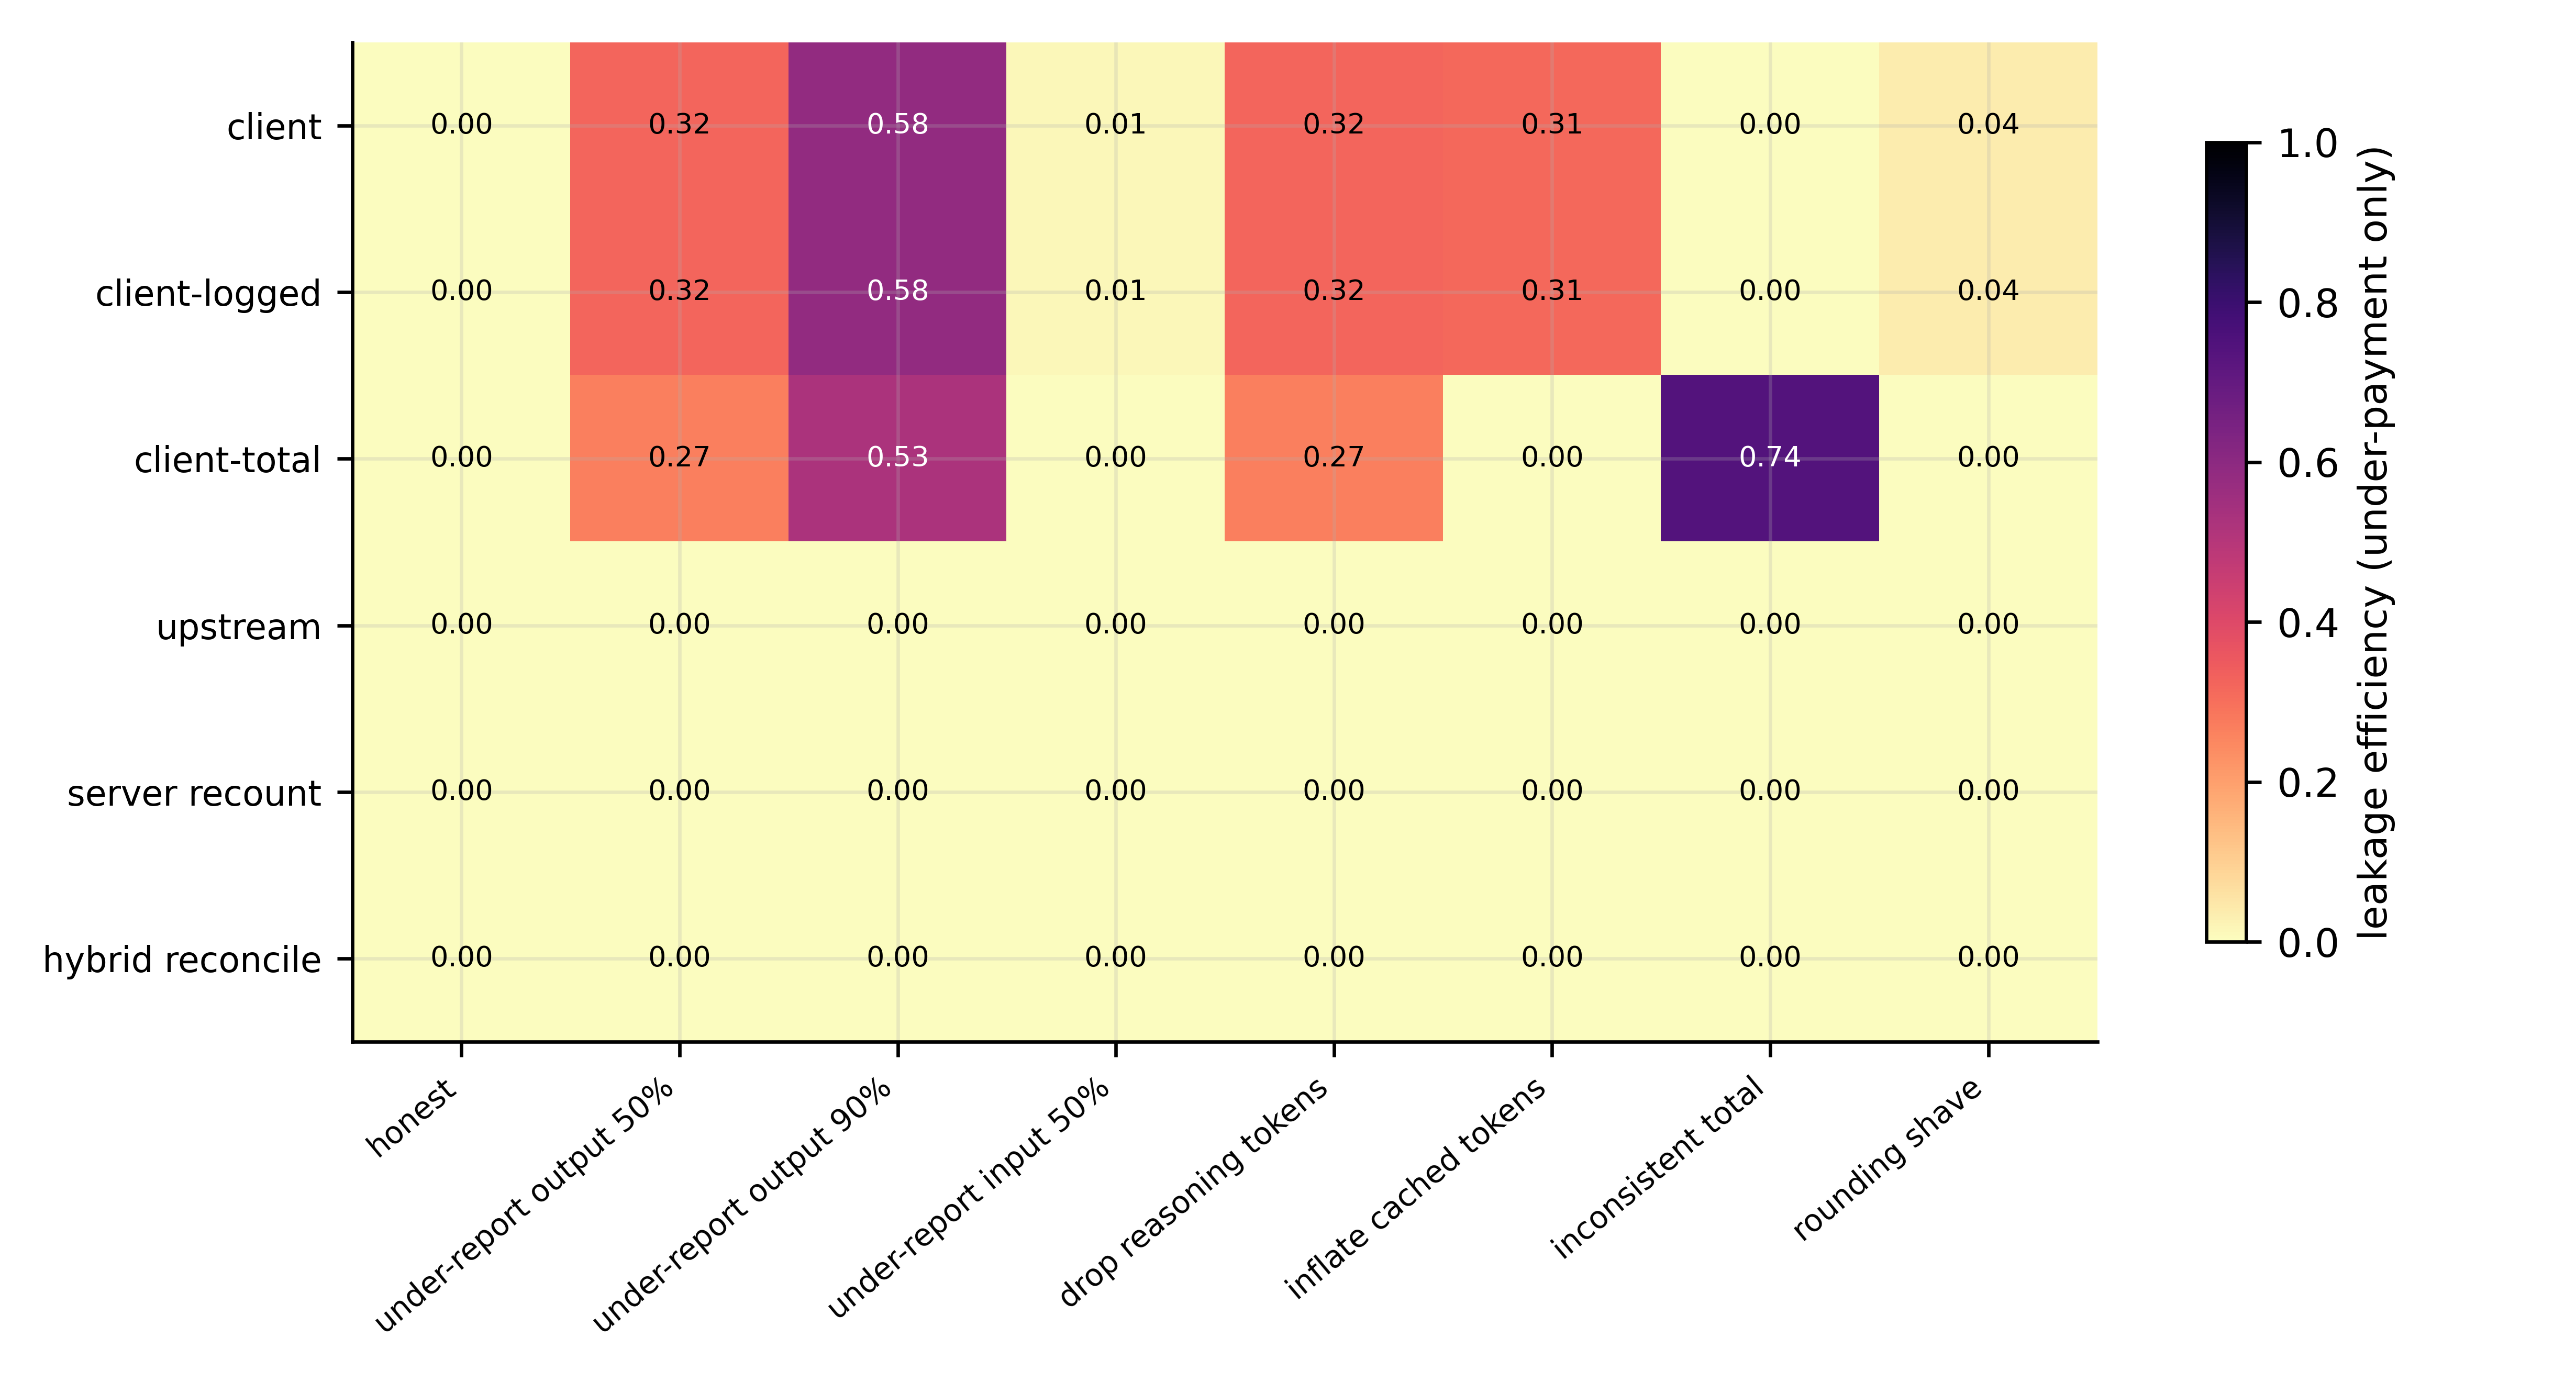
\includegraphics[width=\linewidth]{Figure_5.png}
\caption{M2 leakage efficiency by architecture (rows) against declared-usage
manipulation (columns), deterministic generator, medium tier, concurrency 1, 100
requests/cell. Server-authoritative rows are uniformly zero. The exploitable set differs
between category-additive and flat-total pricing, the empirical form of
Equation~(\ref{eq:m2}).}
\Description[M2 leakage-efficiency heat map by architecture and manipulation]{A six-row
by eight-column heat map compares billing architectures with declared-usage
manipulations. Client-authoritative rows contain nonzero cells, including 0.58 for
90-percent output under-reporting in the client and client-logged rows and 0.74 for an
inconsistent total in the client-total row. The upstream, server-recount, and
hybrid-reconcile rows are zero for all eight manipulations.}
\label{fig:m2}
\end{figure}

\subsection{Lifecycle failure modes}
Beyond the scripted attacks we inject nine lifecycle failures: disconnect at $t=0$ and
mid-stream, truncated stream, settle-window race, missing, delayed, and duplicated usage
metadata, and a recount-engine failure. Every invariant violation falls on a vulnerable
architecture, the hardened architectures survive all of them, and a recount-engine
failure is fail-closed: the request is rejected and nothing is served or billed.

\subsection{Limits of detectability measurement}
\label{sec:detect}
A natural extension of this measurement is whether a leak is detectable after the fact
from retained evidence, distinguishing an invisible leak from one that is merely
unreconciled. We tested this directly and found that our instrumentation cannot support
the distinction.

Two defects were involved. The implementation assigned the detectability level from
static architecture metadata rather than measuring it, so the experiment read back a
label we had set. When we replaced that with a classifier reading only retained ledger
evidence and blind to architecture labels, the distinction disappeared: the two
architectures in question retain identical evidence, so both are equally reconcilable.
Across the full dataset, 2{,}200 records carrying the stored ``invisible'' label are
reconcilable or prevented on the evidence, and no record in the study qualifies as
invisible at all.

The root cause is a property of the testbed rather than of the architectures: our
harness records ground-truth usage for every architecture because it needs that value to
compute leakage, whereas a production deployment need not retain it. Our instrumentation
therefore cannot distinguish detectability classes, so we make no detectability claim. We
report this as a limitation rather than build additional instrumentation to rescue the
metric.

\section{Defenses and Sufficiency Conditions}
\label{sec:sufficiency}
The ablation shows which primitive is load-bearing empirically. Here we state, per
mechanism, conditions sufficient within the accounting model to guarantee
Equation~(\ref{eq:integrity}). These are model-level arguments, not universal theorems
about deployed systems, and we keep what the model forces separate from what our
implementation happens to supply.

\paragraph{M1, commitment timing}
Two conditions suffice. (M1-a) Terminal-path totality: every terminal path (client
disconnect, server exception, stream truncation) reaches a state where an accounting
event for $r$ is committed and durable. (M1-b) Refund boundedness: every refund satisfies
Equation~(\ref{eq:refund}). If a reservation was taken, (M1-b) gives $N(r) =
\mathrm{Res}(r) - F(r) \ge V(r)$; if not, (M1-a) forces the terminal event to commit
$D(r) = V(r)$. Solvency is a separate condition, (M1-c): reserve atomically before
execution and refuse the request when the reservation fails. The no-reserve-settle
ablation cell satisfies (M1-a) and (M1-b) but not (M1-c), and measured exactly that:
integrity held while the balance went negative.

\paragraph{M2, usage authority}
Two conditions suffice. (M2-a) Authority: the usage value used for billing derives from
state the attacker cannot control, $U_{\mathrm{bill}} = U_{\mathrm{true}}$. (M2-b)
Pricing monotonicity: $P$ is non-decreasing in each category. Computing $U_{\mathrm{true}}$
is not sufficient. An architecture that computes it correctly, records it, and bills
$P(U_{\mathrm{decl}})$ satisfies ``the server recounts'' while violating (M2-a), and
leaks $P(U_{\mathrm{true}}) - P(T(U_{\mathrm{true}}))$.

\paragraph{B0, synchronization}
(B0-a): the authorization decision must be atomically coupled to the economic commitment
on the path that authorizes service (Section~\ref{sec:statemodel}) -- a condition about
\emph{where} in the pipeline the atomic operation sits, not merely that one exists.
Concurrency is one way to break that coupling; delayed settlement
(Section~\ref{sec:generality}) is another, requiring no concurrency at all.

\paragraph{Implementation-specific caveats}
The model says ``committed and durable''; our implementation achieves it with a
cancellation-shielded settlement task, and a framework that cancelled that task would
satisfy the architecture on paper while violating (M1-a). The upstream architecture
satisfies (M2-a) only because the provider is honest by assumption. And (B0-a) is a
property rather than a mechanism: our backends obtain it by a conditional \texttt{UPDATE}
and by an anchor-row lock respectively, which is what Section~\ref{sec:generality} tests.
The asynchronous family's own durability caveat is separate from all three: the queued
settlement event itself needed a durable record independent of the message queue, which
Section~\ref{sec:outboxdurability} describes; that fix was validated against the specific
failure points we injected (worker termination before, during, and after consumption;
hard termination of the queue process; duplicate delivery) and not against arbitrary-scale
distributed failure or a host restart.

\subsection{Practical guidance}
Table~\ref{tab:practical} condenses the analysis into what an operator can act on.

\begin{table}[t]
\caption{Practical defense summary. The model-level condition is what the accounting
model requires; the implementation pattern is what we built and measured. Satisfying the
pattern in a different system does not by itself establish the condition there.}
\label{tab:practical}
\centering
\resizebox{\linewidth}{!}{%
\renewcommand{\arraystretch}{0.92}%
\begin{tabular}{lp{3.6cm}p{2.1cm}p{4.3cm}p{5.0cm}}
\toprule
Mech. & Failure mode & Property at risk & Model-level condition & Implementation pattern \\
\midrule
B0 & Authorization reads credit state before prior commitments land &
Ledger conservation, solvency &
Authorization atomically coupled to economic commitment on the authorizing path &
Conditional \texttt{UPDATE ... WHERE balance >= cost} evaluated on the request path, not
deferred to a later worker \\
M1 & A terminal path exits without a committed debit, or over-refunds the unconsumed
reservation &
Accounting integrity; solvency separately &
Terminal-path totality plus refund boundedness (Eq.~\ref{eq:refund}); reservation for
solvency &
Cancellation-shielded settlement on every exit path, refund capped at
$\mathrm{Res}(r) - V(r)$, atomic reserve before execution \\
M2 & Correct usage is computed and stored, but billing reads a client-influenced
representation &
Accounting integrity &
Billing basis derived from state outside attacker control; pricing monotone per category
&
Server-side recount used as the billing input, with the declared vector retained only
for reconciliation \\
Async & Usage event lost, duplicated, or applied after the next authorization &
Accounting integrity; conservation &
Durable, idempotent accounting events with bounded reconciliation lag &
PostgreSQL transactional outbox: settlement event committed durably in the same
transaction as the accounting record, before reaching the queue; idempotency key per
event; at-least-once delivery with duplicate suppression; queue-independent
reconciliation recovers any event the queue fails to deliver \\
\bottomrule
\end{tabular}}
\end{table}

\subsection{What the strongest M2 defense costs}
We measure the M2 recount at three levels because they answer different questions,
reporting the noise band alongside the measured ratios per standard concerns about
benchmarking rigor \citep{kalibera} and measurement bias from innocuous setup choices
\citep{mytkowicz}.

First, the standalone tokenizer (Figure~\ref{fig:toklat}). Cost is linear in input
length (log--log slope 0.999 to 1.14 with $R^2 \ge 0.998$), so it budgets as tokens
times a per-token constant, roughly 0.7\,$\mu$s/token for tiktoken and 2.5\,$\mu$s/token
for SentencePiece. At 16{,}384 tokens the engines span 10.1 to 41.8\,ms, a 2.9 to
3.6$\times$ implementation effect, and at fixed token count the workload alone changes
cost by up to 3.4$\times$.

Second, the gateway with the deterministic generator. Recount is nearly free at 1{,}024
tokens or fewer, retaining at least 0.96$\times$ throughput, but costs heavily at
16{,}384 tokens, at 0.05 to 0.76$\times$. Tokenization time explains this, with Spearman
rank correlation \citep{spearman} $\rho = -0.868$ and $p = 1.3 \times 10^{-5}$.

Third, the local real-model experiment. With real autoregressive generation the recount
is well under 0.1\% of end-to-end time across 128-, 1024-, and 4096-token contexts: 0.014
to 0.019\% at 64 new tokens, and 0.017 to 0.028\% on an independent re-measurement with
separately written timing code at 32 new tokens. The ratio rises as generation shortens,
which is what the cost model predicts. Measured throughput ratios scatter around 1.0 with
signs that flip across workloads, inside a $\pm$10\% noise band that is itself some
700$\times$ larger than the effect.

The apparent expense in the second case is an artifact of a free generator: when
generation costs nothing, tokenization is the entire request. We report all three rather
than the most convenient one -- the recount is not free, but a real, predictable cost
small relative to real inference in the tested configuration.

\begin{figure}[t]
\centering
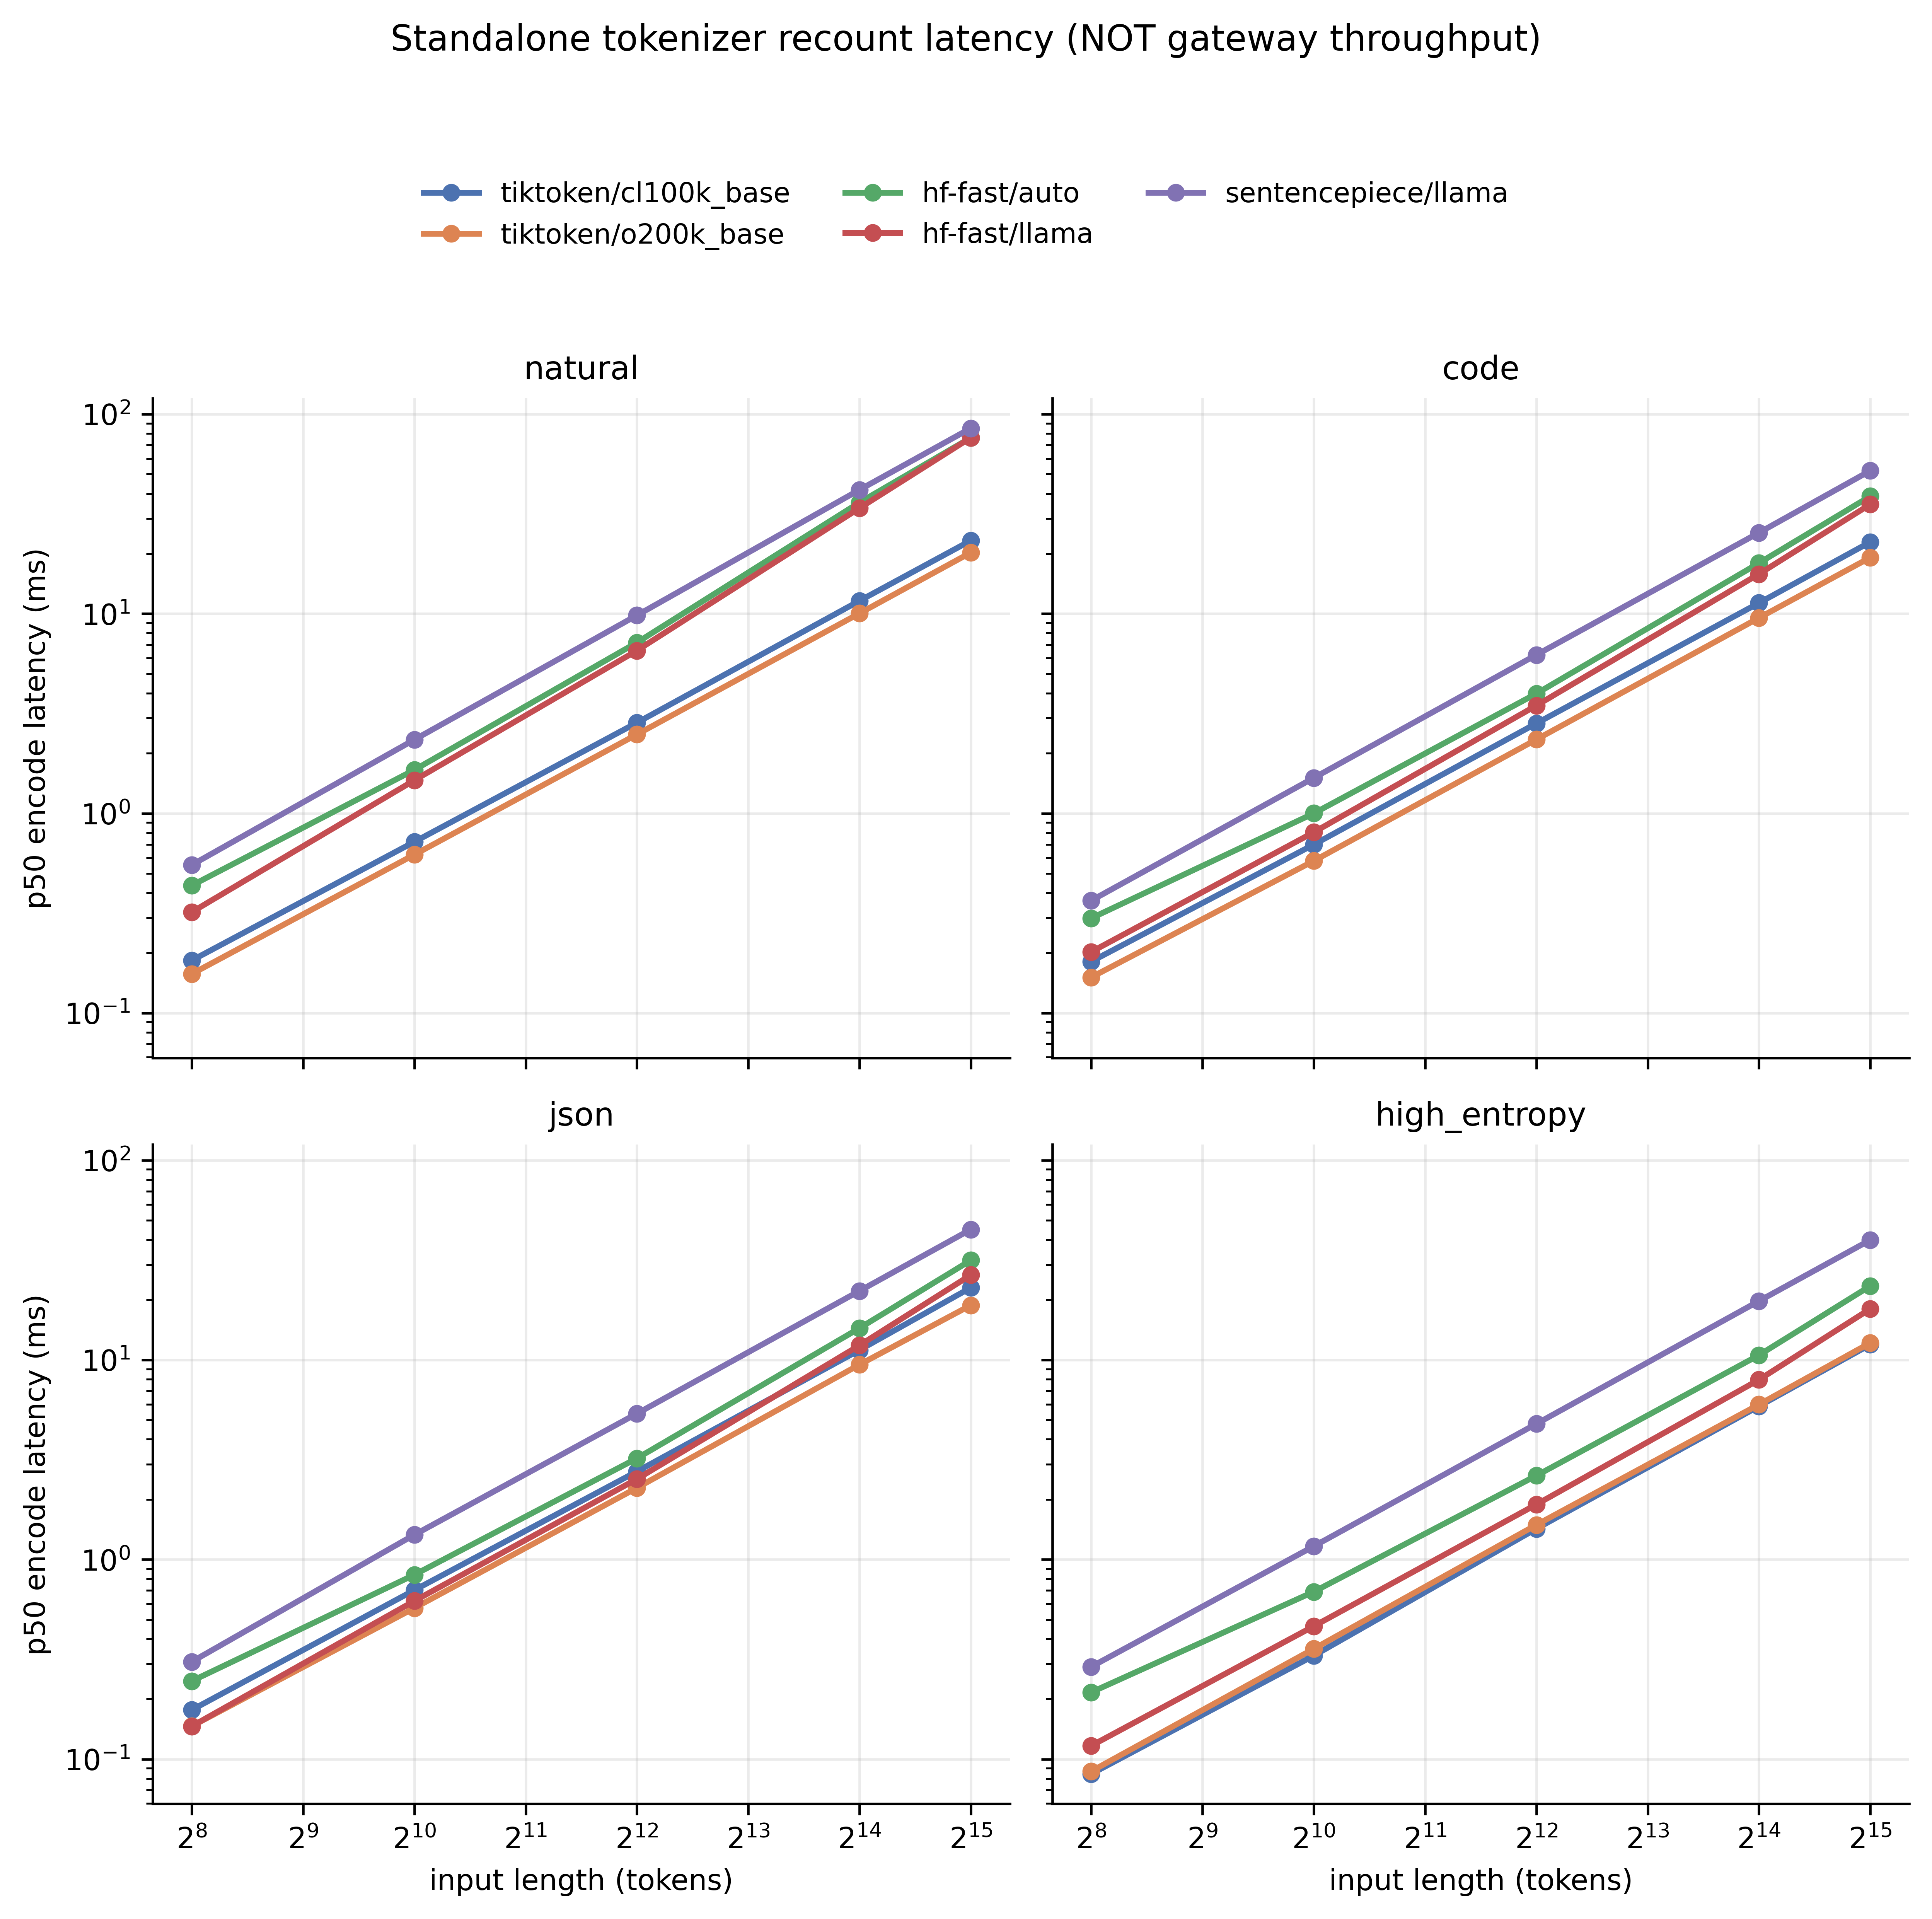
\includegraphics[width=\linewidth]{Figure_6.png}
\caption{Standalone tokenizer recount latency (p50, log--log axes) by engine and input
length, across four text workloads (natural prose, source code, JSON, and
high-entropy/random text), over 100 cells whose token lengths were verified exactly.
Cost is linear in input length within every workload, so recount budgets as tokens times
a per-token constant; the workload shifts the constant, not the linear shape. This is a
tokenizer microbenchmark, not a gateway throughput result: no request path, database, or
network is involved.}
\Description[Tokenizer recount latency grows linearly with token count]{Four log-log line
charts show natural-language, source-code, JSON, and high-entropy workloads. Each chart
compares five tokenizer engines from 256 to 32768 input tokens. Every engine forms an
approximately straight rising line, indicating linear scaling with token count. The
SentencePiece Llama engine is consistently the slowest; the two tiktoken engines are
generally fastest, while workload changes the vertical spacing between engines.}
\label{fig:toklat}
\end{figure}

\section{Cross-Architecture and Asynchronous Validation}
\label{sec:generality}
A measurement study on one deployment invites the objection that its conclusions are
deployment artifacts. We repeated the experiments while changing only the deployment, the
storage architecture, or the inference data plane; the attack harness, the architectures
under test, and the integrity gates stay identical across all runs. Each varied dimension
(execution topology, accounting backend, inference data plane, settlement architecture)
tests whether an observed behavior belongs to the architecture or to one implementation
of it.

\subsection{Execution topologies and accounting backends}
Three topologies: a single uvicorn worker with no proxy, as control; nginx over four
uvicorn workers, giving four independent event loops sharing one PostgreSQL and one
Redis; and an nginx load balancer over two gateway containers. Across 96 accounting
cells there were no mismatches against the control. Two genuine multi-worker defects
surfaced during this work and are reported rather than hidden: the B0 runtime posture was
per-process and would have reached one worker in four, and concurrent schema creation
raced. Both were fixed.

Backend A keeps a mutable balance row and obtains atomicity from a conditional
\texttt{UPDATE ... WHERE balance >= cost}. Backend B never mutates that row: every
movement is an immutable entry in an append-only ledger and the balance is derived as the
sum of entries, with the atomic reserve becoming a conditional append serialized on an
anchor row.

All 17 comparison cells agreed, and we state plainly what that number contains. Only
eight genuinely exercised both backends. Five agree for an analytic reason: the M2
billed amount is computed before any balance is read, so it cannot vary by backend.
Four are B0 cells whose frozen debit module contains no reference to the backend
abstraction, so they ran identical code twice. The defensible statement is that eight
genuine backend-sensitive cases agreed and none disagreed. B0's independence from the
storage representation is therefore untested, and we list it as a limitation.

\subsection{A real serving stack}
\label{sec:realstack}
Every figure so far was produced against a generator we wrote. That is what makes the
accounting arithmetic exact, but it leaves an obvious objection open, so we repeated the
experiments with the token source replaced by llama.cpp's server \citep{llamacpp} running
SmolLM2-135M-Instruct \citep{smollm2} on CPU. This is self-hosted serving code we did not
write, with a real subword tokenizer, real server-sent event streaming \citep{sse}, and
usage records the server produces itself. The gateway, architectures, accounting
backends, settlement logic, and integrity gates are unchanged, and the deterministic
default remains byte-identical, with both regression suites still passing.

Across 12 M1 cells and 48 M2 cells there were no safety disagreements. Vulnerable
commitment-timing architectures still leak on abort and collapse to zero at completion,
reserve-and-reconcile still leaks nothing, and every server-authoritative architecture
still leaks exactly 0.000 across all eight manipulations.

Attack effectiveness did move, and we report it rather than average it away. Output
under-reporting at 90\% yields 0.690 here against 0.583 on the deterministic generator,
because SmolLM2 emits no reasoning tokens and output therefore dominates the cost. For
the same reason the K2 manipulation that drops hidden reasoning tokens becomes completely
inert: there is nothing to drop. Under flat-total pricing three cells flip sign, because
on this token mix flat-total overcharges by so much that even a 90\% under-declared total
still exceeds the authoritative category cost. Five of the 48 cells changed effectiveness
in total; the per-cell comparison against the deterministic corpus is in the released
artifact. The architectural conclusion is generator-independent; the per-manipulation
magnitudes are not.

Real serving also exhibits a property the deterministic generator cannot: the server reports
a prefix-cache split, and because cached input is priced an order of magnitude below
uncached input, the honest charge for a byte-identical request depends on server cache
state. Repeating identical requests, the reported split moved (24 then 52 of 53 prompt
tokens in one instance) and the authoritative cost moved with it by 22 to 27\%, reaching
32\% at the extreme, on all three prompts tested. This sharpens the threat model -- a
client cannot verify its own bill even in principle, and over-declaring cached tokens
carries genuine plausible deniability since the true value legitimately varies -- though
it is one stack with one prefix-cache implementation, not generalized to hosted APIs.

\subsection{Asynchronous accounting}
\label{sec:async}
Both backends so far settle before the response completes. Real metering pipelines
often do not: the gateway emits a usage event and a separate worker applies it later. We
therefore added a third accounting family, an event queue with a continuously running
worker and a controlled reconciliation delay $D$, because a claim of architectural
generality that quietly assumes strong consistency is not worth much.

With an honest pipeline, asynchronous accounting is delayed rather than lossy. The mean
exposure window between value delivery and durable debit tracks $D$ closely: at $D = 0,
10, 50, 100, 500$\,ms the measured windows are 14.0, 14.9, 54.3, 103.7, and 504.1\,ms, and
the leak reconciles to exactly zero. Duplicated events are suppressed idempotently across
all 25 injected duplicates. A lost event, by contrast, leaks permanently at every delay.
This is an injected application-level fault (the event is never created), distinct from
the infrastructure-level queue failure discussed in Section~\ref{sec:outboxdurability}, and
the result above is unaffected by that section's fix. Whether a straggler looks lost or
merely late is a property of the observation horizon
rather than of the architecture; we used four times the configured delay, floored at
400\,ms, and the released artifact records the per-cell outcome. The reconciliation
delays used here are injected experimental parameters, not delays observed in a
production pipeline.

\subsection{B0 revisited: the condition is not fundamentally about concurrency}
\label{sec:b0revised}
The asynchronous family changed one of our own conclusions, and it is the sharpest
systems result in the paper.

We issued requests strictly sequentially, 20\,ms apart, so that no two were ever in
flight together. We use ``sequential'' throughout this paper in exactly this sense:
arrivals do not overlap, but settlement may still be pending when the next request is
authorized. Section~\ref{sec:netsep} introduces a deliberately different control, strict
serialization of authorization and settlement, which additionally waits for settlement
confirmation and is not interchangeable with the sequential arrivals studied here. Any
over-serving in this experiment therefore does not arise from overlapping in-flight
requests. Over-serving
nonetheless appears once $D$ reaches 100\,ms, and reaches four requests over a
two-request budget at $D = 500$\,ms, with the balance driven negative
(Table~\ref{tab:asyncb0}).

\begin{table}[t]
\centering
\caption{B0 under deferred settlement with strictly sequential arrivals 20\,ms apart, a
two-request budget.}
\label{tab:asyncb0}
\begin{tabular}{lc}
\toprule
Settlement delay $D$ & Requests over-served \\
\midrule
0\,ms & 0 \\
10\,ms & 0 \\
50\,ms & 0 \\
100\,ms & 1 \\
500\,ms & 4 \\
\bottomrule
\end{tabular}
\end{table}

The mechanism is simple once seen. Authorization reads a committed balance that is
correct but stale, because the debits for earlier requests are still in the queue. An
atomic guarded decrement, the entire B0 defense, provides nothing if it lands after
the next authorization has already read the balance. Concurrency was never the essential
ingredient; it was one way of separating the check from the commitment. Delayed
settlement is another, and it needs no concurrency at all.

We therefore restate the B0 condition as given in Section~\ref{sec:sufficiency}:
authorization must be atomically coupled to economic commitment on the path that
authorizes service. This is strictly more general than the concurrency framing we started
with, and the earlier framing was too weak rather than wrong.

M2, by contrast, is untouched: leakage efficiency is identical at 0.5823 at every delay,
confirming the analytic independence of usage authority from settlement timing.

\subsection{Network-separated validation}
\label{sec:netsep}
Every topology in Section~\ref{sec:generality} so far ran on a single host over loopback,
which leaves open whether Section~\ref{sec:b0revised}'s result is an artifact of that
communication path. We repeated the asynchronous B0 experiment with the gateway on one
machine and the accounting store, Redis, and the settlement worker on a second, reached
over the real internet (a cloud VM in a different data center than the gateway host), with
the attack harness, architectures, and integrity gates unchanged.

While building this topology we found that our own sequential-arrival harness had a pacing
confound: it paced requests by sleeping a nominal interval after each full round trip, and
over the real network the round trip itself, not the sleep, dominated the achieved
inter-arrival gap, measured directly from request timestamps at 513--857\,ms rather than
the intended 20\,ms. We fixed the harness to record the achieved gap per request and reran
with a delay range chosen to straddle that measured gap. The corrected sweep
(Table~\ref{tab:twomachine}, $N=6$, budget $k=2$, 5 repetitions per delay) shows a clean
transition: no over-serving through $D=2000$\,ms, partial over-serving at $D=5000$\,ms,
and saturation at $N-k=4$ by $D=10000$\,ms.

\begin{table}[t]
\centering
\caption{Sequential arrivals with deferred settlement over the network-separated
two-machine topology, budget $k=2$, $N=6$. Over-served counts across 5 repetitions per
delay.}
\label{tab:twomachine}
\begin{tabular}{lc}
\toprule
Settlement delay $D$ & Over-served (5 reps) \\
\midrule
0--2000\,ms & 0, 0, 0, 0, 0 \\
5000\,ms & 3, 2, 2, 2, 2 \\
10000\,ms & 4, 4, 4, 4, 4 \\
\bottomrule
\end{tabular}
\end{table}

The B0 mechanism persisted under a network-separated two-machine deployment, while strict
serialization of authorization and settlement produced no observed over-serving across the
tested settlement delays. We distinguish the two deliberately: \emph{sequential arrivals
with deferred settlement} (the mechanism above, and in Section~\ref{sec:b0revised}) means
requests do not overlap but settlement may still be pending when the next request is
authorized; \emph{strict serialization of authorization and settlement} means the harness
confirms, from the account's own authoritative balance, that settlement for request $i$
has completed before request $i+1$ is dispatched. The strict-serial control polls the
authoritative balance until it equals the expected post-settlement value; an earlier
implementation polled the queue's reported depth instead and was replaced after we found a
transient window in which the queue reports empty while an event is still in transit. Over
the same two-machine topology, strict serialization produced zero over-serving in every one
of twelve tested cells ($D \in \{0, 500, 2000, 10000\}$\,ms, 3 repetitions each; served
equaled the budget exactly in all twelve).

This is evidence for one tested topology, one cloud region, and one host pair, not a
characterization of networked deployments in general; Section~\ref{sec:limits} states the
remaining scope precisely.

\subsection{Durability of the queued settlement event}
\label{sec:outboxdurability}
Fault injection during the network-separated work surfaced a second, independent finding
about the testbed's own queue, distinct from the B0 admission race above. Before this fix,
the only record of a pending settlement event was the message in the Redis queue; no
durable record existed until the worker applied the debit. We tested this directly, not by
simulation: we queued an event with its delay not yet elapsed, confirmed it was queued, hard
-terminated the Redis process, restarted it, and found the event permanently lost, with the
queue empty and the corresponding debit never applied.

The fix is a PostgreSQL transactional outbox, described as an implementation pattern in
Table~\ref{tab:practical}: the settlement event is written as a durable row in the same
database transaction as the accounting record, committed before the event is handed to the
queue, so a durable record exists independent of the queue from the moment the request is
admitted. A settlement worker claims and applies an event in one atomic transaction, so no
intermediate state exists in which an event is marked settled without the debit having
landed. A queue-independent reconciliation pass scans for due, unsettled events and applies
them directly from the durable record, recovering anything the queue failed to deliver.

We re-ran the targeted failure points this fix addresses and confirmed each by raw evidence,
not inference: a worker terminated before an event was due recovered correctly on restart
with exactly one debit applied; a hard termination of the queue process after an event was
queued but not yet due was recovered by the reconciliation pass once the event's delay
elapsed, rather than lost; duplicate delivery was suppressed with zero double-charging; and
ledger conservation and final-balance correctness held in every case tested. We did not
force a live database transaction rollback (argued analytically from the single-transaction
design instead) and did not test a virtual-machine or host restart. Delivery remains
at-least-once, not exactly-once: the queue or the reconciliation pass may both attempt to
apply the same event, and the atomic claim ensures duplicate delivery does not result in a
duplicate debit, which is a narrower and verifiable guarantee than claiming no event is ever
delivered twice.

We characterize this architecture precisely rather than with a single adjective: before
the fix it was process-crash vulnerable to termination of the queue process (a permanent
loss, not merely a recoverable delay); after the fix it is eventually durable with
at-least-once delivery and idempotent settlement application, at the specific failure
points tested, and not validated against a host restart, arbitrary-scale distributed
failure, or any topology beyond Section~\ref{sec:netsep}'s own two-machine pair. The fix
changes nothing about the B0 admission race studied throughout this paper -- the race is
in the authorization read, which it does not touch -- and every pre-existing
asynchronous-family experiment (Sections~\ref{sec:async}, \ref{sec:b0revised}) reproduced
identical results when re-run against it, since none inject a queue failure.

\section{Economic and Pricing Analysis}
\label{sec:economics}
The security question in M2 reduces to an economic one. With $U$ the true usage vector,
$T$ the attacker's transformation, and $P$ the pricing function, a manipulation is
profitable exactly under Equation~(\ref{eq:m2}): the pricing basis must read a field that
$T$ changes.

That has an immediate structural consequence. Under category-additive pricing, $P(U) =
\sum_i p_i u_i$, a manipulation pays off if and only if it reduces a category the
function actually reads. Declaring a total inconsistent with the subtotals is therefore
inert, measured at 0.000, because category pricing never reads the declared total. Under
flat-total pricing, $P(U) = p \cdot \mathrm{total}(U)$, the same manipulation becomes the
strongest attack in the catalog at 0.741, while reclassifying output into a discounted
cached category becomes inert because no category is read at all. Mixed pricing over
input, output, cached, and reasoning categories sits between the two, and its exploitable
set is determined by which categories carry distinct prices.

Two kinds of price change must be distinguished. Uniform scaling of every price by a
constant leaves leakage efficiency unchanged (confirmed across a $10\times$ scaling in
the full price-tier sensitivity table, released in the artifact), which is why we use
efficiency as the headline metric and label absolute dollars as scenario values.
Structural repricing -- changing the ratios between categories, or moving between
category-additive and flat-total bases -- changes which transformations are profitable,
and can change them qualitatively: the real-stack experiment demonstrates this directly,
where three flat-total cells reverse sign on a token mix with no reasoning tokens because
the pricing basis overcharges by more than the manipulation evades.

The pricing tiers used in our experiments are synthetic; Table~\ref{tab:pricing} shows
one provider's published list prices only to establish that such wide,
category-differentiated ratios are current commercial practice, not a construction of
ours.

\begin{table}[t]
\caption{Published list prices for one commercial provider, as an example of
category-differentiated pricing in current practice \citep{anthropicpricing}. Reproduced
for context only; this paper makes no claim about any provider's metering or accounting
implementation, and no commercial service was tested.}
\label{tab:pricing}
\centering
\resizebox{\linewidth}{!}{%
\begin{tabular}{lrrrr}
\toprule
Model & Input & Cached input & Output & Cached : input \\
 & (\$/Mtok) & (\$/Mtok) & (\$/Mtok) & \\
\midrule
Sonnet 5   & 2 & 0.20 & 10 & 0.10 \\
Haiku 4.5  & 1 & 0.10 & 5  & 0.10 \\
Opus 5.5   & 4 & 0.20 & 20 & 0.05 \\
\bottomrule
\end{tabular}}
\end{table}

We deliberately stop short of a revenue-impact model: estimating aggregate exposure would
require assuming an attacker population and request volume, and the result would be
invention dressed as measurement. What the analysis supports is a design rule: the
pricing basis determines the attack surface and should be chosen with that in mind, not
for billing convenience alone.

\section{Discussion}
\label{sec:discussion}
Three dimensions of one accounting boundary behave differently because each is defective
in a different element of the lifecycle: B0 is a shared-state property that fails
whenever the check is separated from the commitment, while M1 and M2 are per-request
properties with no concurrency dependence in the tested design
(Sections~\ref{sec:taxonomy} and~\ref{sec:results}).

The practical consequences are three: an operator cannot use traffic level as a proxy for
exposure, since two of the three dimensions do not scale with load at all and the third
fails under sequential arrivals if settlement lags; integrity and solvency need different
controls, so a system with only one will look correct in whichever dimension it is
measured; and in the evaluated architectures a correct recount did not prevent leakage
unless authoritative for billing. The defenses themselves are ordinary; the contribution
is knowing which one is load-bearing, and what it costs.

\paragraph{Engineering implications}
Within the tested and modeled conditions, the results place each control at a specific
architectural location. Authorization belongs on the same path as the economic
commitment it depends on, not on a deferred worker, because an atomic decrement that
lands after the next authorization has read the balance provides nothing. The billing
input belongs to state outside attacker control, so the recount that feeds billing must be
authoritative rather than merely computed. Every terminal path of the request lifecycle
must reach a durable accounting event -- a cancellation-shielded settlement task for M1,
and the transactional outbox of Section~\ref{sec:outboxdurability} for the asynchronous
family's queued event. The implementation patterns we built are not
equivalent to the model-level conditions: satisfying a pattern in another system does not
by itself establish the condition there, which is why Table~\ref{tab:practical} keeps them
apart. These are implications for engineering metered services under the stated
accounting model, demonstrated on LLM inference; Section~\ref{sec:limits} states the
scope precisely.

\paragraph{Relation to known weakness classes}
This is the objection we consider most likely, so we state it ourselves: the individual
mechanisms have precedents in isolation (Sections~\ref{sec:related}
and~\ref{sec:deployed}), B0 is a known race presented as a baseline, not a contribution,
and we claim no novelty at the primitive level.

Beyond these known primitives, the paper adds the unification stated in the contributions
list (Section~\ref{sec:intro}), plus two things no primitive-level description predicts:
the M1 ablation shows, by exhaustive model
checking rather than by example, that solvency and accounting integrity are orthogonal
and need different primitives, which ``there is a streaming bug'' does not predict; and
the M2 ablation shows an architecture that recounts usage correctly can still leak if
billing is not authoritative. We do not assert practitioners believed a recount was
sufficient; we show experimentally that in the evaluated architectures it was not.

\section{Threats to Validity}
\label{sec:limits}
We organize threats as internal, construct, external, and formal
validity \citep{runeson,wohlin}, and add one for the
degree of physical distribution actually exercised.

\paragraph{Internal}
A single uvicorn worker in the base configuration makes gateway recount numbers an upper
bound; the host is shared and Docker scheduling is not controlled. Local loopback adds a
roughly 45\,ms floor per request, making the gateway ratios conservative for small
inputs. Leakage that depends on delivered tokens is sensitive to
disconnect timing at high concurrency: the within-cell standard deviation of delivered
tokens is exactly zero at concurrency 20 or below and about 0.011 at 50 and 100.

\paragraph{Construct}
The B0 debit path is a frozen module predating the pluggable accounting backends, so
backend parity covers M1 and M2 only and B0's storage independence is untested. Our detectability instrumentation restates
experimenter-assigned labels rather than measuring evidence, so we make no detectability
claim.

\paragraph{Formal}
Evidence labels, proof scope, and what neither specification claims are stated in
Section~\ref{sec:formal} and apply here. The primary specification is
finite (two to three concurrent requests, two value chunks, unit pricing) and assumes
strongly consistent accounting state, so it does not cover the asynchronous family. The
second specification (Section~\ref{sec:asyncformal}) covers the asynchronous-settlement
mechanism as an untimed, causal-ordering abstraction, with no notion of milliseconds,
network behavior, or database semantics, checked at six finite $(N,k)$ points. Neither
specification models multi-category pricing or tokenizer disagreement.

\paragraph{External}
The empirical scope is one controlled testbed, one llama.cpp/SmolLM2 stack, one small
model on CPU, and one prompt family: this shows the
architectural conclusions are not artifacts of our own generator, but not behavior on
commercial providers -- the cache-split nondeterminism is a property of this stack's
prefix cache, not a claim about hosted APIs. The generator-dependent cells bound how far
per-manipulation magnitudes travel. Reconciliation delays are injected, not observed in
production, so the asynchronous result is conditional: if settlement lags authorization by
more than the inter-arrival time, atomicity on the settlement path does not prevent
over-serving. Pricing tiers are synthetic. More broadly, the experiments show the modeled
accounting failures are realizable under the specified architectures and workloads; they
do not show any particular commercial provider implements them, that they are prevalent
across deployed LLM services, or that a specific provider is vulnerable. Public issue and
pull-request evidence cited here shows only that related behaviors are reported in
deployed and open-source infrastructure, not a claim about any named system's current
state. It does not establish production prevalence. The preregistered 1,200-trial
terminal-path fault matrix was not executed because the local Docker daemon was
unavailable; it remains a protocol, not a result.

\paragraph{Distribution}
Separation in the topology experiments of Section~\ref{sec:generality} (execution
topologies, accounting backends) is temporal, not physical: those topologies ran on a
single host under Docker Compose over loopback. The asynchronous settlement family was
also run with the accounting store, Redis, and settlement worker on a second machine
reached over the real internet (Section~\ref{sec:netsep}); the condition persisted there,
so it is not an artifact of loopback communication specifically. This narrows but does
not remove the limitation: we tested one cloud-region
host pair, not network partition, clock skew, or cross-machine queueing behavior in
general, and we did not test a VM or host restart, a wide-area or multi-region topology,
or a production deployment. No independent second-host replication was executed in this
upgrade: the discussion above concerns the preserved author-run dataset, whose raw records
and manifests were inspected, not a fresh external validation.

\section{Responsible Disclosure and Ethics}
This work produced no new vulnerability findings against any third-party, live, or
production system: all experiments ran against the local testbed shipped with the
released artifact, whose harness defaults to \texttt{localhost} and contains no
third-party endpoints, and no credentials, real user data, or production billing APIs
were used. The public artifacts cited as prior evidence in Section~\ref{sec:deployed}
were public, and in two cases already fixed, before this work; they are reports by those
projects' own maintainers and users, not findings of ours, and we reviewed only their
published issue and pull-request pages. Every attack in the artifact is paired with a
defense, and the testbed is released so operators can measure their own gateways.

\section{Conclusion}
This paper is an evidence-backed security study of accounting integrity in metered
AI-serving infrastructure, using LLM inference serving as the concrete deployed-system
workload. Client-side under-payment
is best modeled as one accounting boundary with three placements: synchronization,
commitment timing, and usage authority. Localizing each to a state transition predicts,
and our measurements confirm, that integrity and solvency are closed by different
primitives and a server-side recount must be authoritative, not merely computed.
Exhaustive model checking establishes
the M1 orthogonality over all four combinations rather than the two we implemented, and
the same checking refuted our first specification before it confirmed the corrected one.

The result we did not expect concerns the baseline: B0 began, in this implementation, as
a concurrency race, but the asynchronous experiment showed concurrency was incidental to
the underlying failure -- what matters is whether authorization is atomically coupled to
economic commitment on the path that authorizes service. Delayed settlement breaks that
coupling with no concurrency whatsoever. The corrected condition is more general than the
one we started with, and is the form an operator should test against. In the tested configuration the strongest M2 defense costs a small and
predictable fraction of real inference time; B0's atomic decrement and M1's
reserve-reconcile path are not characterized by this same cost measurement.

\section*{Acknowledgements}
No external acknowledgements apply to this work.

\section*{Author Contributions}
\textbf{Hardik}: Conceptualization, Methodology, Software, Investigation, Formal
analysis, Data curation, Validation, Visualization, Writing -- original draft, Writing --
review and editing. \textbf{Natasha Kaila}: Investigation, Writing -- review and editing.

\section*{Declaration of competing interest}
The authors declare that they have no known competing financial interests or personal
relationships that could have appeared to influence the work reported in this paper.

\section*{Funding}
This research received no specific grant from any funding agency in the public,
commercial, or not-for-profit sectors.

\section*{Data availability}
Source code, the attack harness, defense implementations, the TLA+ specification, and all
raw experimental data are released at
\url{https://github.com/meowlawat/TOKEN-ACCOUNTING-INTEGRITY-IN-LLM-METERING}, tagged
release \texttt{v1.1.0}, which is the version reported in this paper, including the
network-separated validation and strict-serialization control (Section~\ref{sec:netsep}),
the transactional-outbox durability fix (Section~\ref{sec:outboxdurability}), and the
second, asynchronous-settlement formal model (Section~\ref{sec:asyncformal}). Tags
\texttt{v1.0.0} and
\texttt{v1.0.1} are preserved unchanged as earlier historical snapshots that precede this
manuscript's additions and do not contain them; \texttt{v1.0.1} differs from
\texttt{v1.0.0} only in how the B0 condition is stated and in no measured value. The
complete artifact (source code, experiment scripts, both TLA+ specifications, raw and
processed results, figures, tables, and reproduction scripts) corresponding to this
version is archived in Zenodo under the concept DOI
\href{https://doi.org/10.5281/zenodo.22085827}{10.5281/zenodo.22085827}, which always
resolves to the most recent archived version, and under version DOI
\href{https://doi.org/10.5281/zenodo.23261555}{10.5281/zenodo.23261555} specifically, the
version corresponding to GitHub tag \texttt{v1.1.0}. An earlier version DOI,
\href{https://doi.org/10.5281/zenodo.22086254}{10.5281/zenodo.22086254}, archives the
artifact at tag \texttt{v1.0.1} and remains resolvable as the historical record. The
deposited archive's contents and checksum are listed in \texttt{release/zenodo/} in the
repository.

\bibliographystyle{ACM-Reference-Format}
\bibliography{references_taisap}

\end{document}
